\documentclass[
a4paper,
twoside,
DIV=calc,
BCOR=4mm,
fontsize=9pt,
twocolumn=on,
titlepage=on,
parskip=half
]{scrartcl}
\usepackage{german,supertabular,graphicx,hyperref,pbox}
\usepackage[utf8]{inputenc}
%\usepackage[T1]{fontenc}
%\usepackage{helvet}
%\usepackage{mathphv}

\usepackage{float}
\floatstyle{boxed}
\restylefloat{figure}

%\renewcommand{\familydefault}{phv}
%\renewcommand{\familydefault}{cmss}
%\setlength{\columnsep}{7mm}

%\usepackage{anysize}
%          {left}{right}{top}{bottom}
%\marginsize{2.0cm}{2.0cm}{2.0cm}{2.0cm}
%\setlength{\footnotesep}{5mm}

\hyphenation{NSpF}
\hyphenation{Re-gel-mo-di-fi-ka-tio-nen}
\hyphenation{Bai-Sse-Yuen}

\newcommand{\midgard}{\textsc{Midgard}}

\author{Bj"orn~Rabenstein\\\href{mailto:bjoern@rabenste.in}{\nolinkurl{bjoern@rabenste.in}}}
\title{Bester Ginseng aus Yü}
\subtitle{\midgard-Abenteuer für 3--5 SpF der Grade 1--3}

\publishers{\fbox{%
\parbox{\columnwidth}{%
Dieses Material steht unter der Creative-Commons-Lizenz \emph{Namensnennung
-- Nicht-kommerziell -- Weitergabe unter gleichen Bedingungen 4.0
International}. Um eine Kopie dieser Lizenz zu sehen, besuchen Sie
\url{http://creativecommons.org/licenses/by-nc-sa/4.0/}.
}%
}}


\begin{document}

\maketitle

\tableofcontents

\section{Einleitung}

Im Januar 2015 erfüllte ich mir so eine Art Jugendtraum und begann,
eine KanThaiPan-Kampagne zu leiten, in deren Zentrum die "`vier
Klassiker"', also die vier Richter-Di-Abenteuer, stehen sollten. Ein
Vorteil der späten Traumerfüllung war, daß wir wirklich mit dem
\emph{Fall des Mondloses} anfangen konnten. Dadurch stellte sich aber
die Frage, wie wir die gut zehnjährige Lücke zwischen dem
\emph{Mondlos} und den \emph{Füchsen} überbrücken sollten. Selbst mit
einem bißchen Füllmaterial und Tricks blieb bei uns eine Lücke von
2392\,nL bis 2400\,nL. Schickte man die SpF wirklich so lange auf
Abenteuer aus, dann wären sie danach so ca. auf Gr9, was dann doch
etwas heftig wäre für den Rest der Kampagne, ganz abgesehen mal davon,
wie lange man dafür bräuchte. Natürlich hätte ich jetzt die SpF acht
Jahre lang ihrem "`normalen"' Leben nachgehen lassen können, oder ich
hätte die Geschichte umschreiben können und die anderen
Richter-Di-Abenteuer früher stattfinden lassen. Beide Möglichkeiten
fand ich aber aus verschiedenen Gründen unbefriedigend. So habe ich
aus der Not eine Tugend gemacht und dieses Abenteuer entworfen, wo als
Teil der Handlung die SpF einen Zeitsprung unternehmen werden, und das
sogar ohne die naheliegende \emph{Macht über die Zeit}, sondern unter
Ausnutzung bekannter Eigenschaften des Multiversums.

Um mit dieser Klappe gleich noch ein paar andere Fliegen zu schlagen,
passieren noch ein paar andere Dinge:

\begin{itemize}
\item Die SpF lernen Ming kennen, den wichtigen Protagonisten aus
  \emph{Kurai-Anat, das Schwarze Herz}. Das ermöglicht es, später den
  Kernteil dieses Abenteuers auch mit einer reinen KanThai-Gruppe zu
  spielen. Ein paar Szenen aus dem Abenteuer, die sonst gar nicht mehr
  zur Geltung kämen, können hier auch gleich verwurstet werden.
\item In den \emph{Perlen der Füchse} schmuggelt der \emph{Weiße
    Lotus} Gingseng in weitem Bogen von irgendwo am Schattenmeer durch
  Minangpahit über den Seeweg nach KuenKung. Dabei liegt doch der
  Hauptproduzent von Gingseng, die Provinz Yü, mehr oder weniger
  direkt vor den Toren der Stadt. Dieses Abenteuer liefert eine
  Erklärung, wie es dazu kommen konnte. Obendrein erfährt man ein
  wenig über das Verhältnis zwischen \emph{Weißer Orchidee} und
  \emph{Weißem Lotus}. Letzterer war ja zu Beginn des Abenteuers noch
  keine eigenständige Geheimgesellschaft, sondern lediglich eine Loge
  von ersterer.
\end{itemize}

Ich kann mir vorstellen, daß auch andere Gruppen in der gleichen
Situation stecken. Daher habe ich mich entschlossen, das Abenteuer
hiermit der Allgemeinheit zur Verfüngung zu stellen. Ich bitte, den
etwas rohen Ausarbeitungszustand zu verzeihen. Ich habe im
wesentlichen auf die Schnelle meine Notizen ausformuliert. Karten und
Skizzen sind in dem beklagenswerten Zustand eingescannt worden, in dem
sie mein bescheidenes manuelles Zeichentalent hinterlassen hat.

Ein Spielbericht meiner Gruppe findet sich unter
\url{http://rabenste.in/kwiki/index.php5/Di002}.

Verweise auf Regelbücher, das KanThaiPan-Quellenbuch und diverse
Abenteuerhefte erfolgen nach dem Schema [\emph{XXX n}], wobei
\emph{XXX} die Abürzung für das Buch bzw. Heft ist (siehe folgende
Liste) und \emph{n} die Seitenzahl im jeweiligen Werk.

\begin{description}
\item[ARK] \emph{Das Arkanum} -- \midgard-Regelwerk 4. Auflage.
\item[BES] \emph{Das Bestiarium} -- \midgard-Regelwerk 4. Auflage.
\item[DFR] \emph{Das Fantasy-Rollenspiel} -- \midgard-Regelwerk 4. Auflage.
\item[DSH] \emph{Kurai-Anat, das Schwarze Herz} -- Abenteuer.
\item[HdB] \emph{Die Haut des Bruders} -- Abenteuer.
\item[KOM] \emph{Das Kompendium} -- \midgard-Regelwerk 4. Auflage.
\item[KTP] \emph{Unter dem Schirm des Jadekaisers} -- Quellenbuch
  KanThaiPan 2. Auflage.
\item[MdS] \emph{Meister der Sphären} -- \midgard-Regelwerk 4. Auflage.
\item[MSS] \emph{Mord am Schwarzdorn-See} -- Abenteuer.
\item[PdF] \emph{Die Perlen der Füchse} -- Abenteuer.
\end{description}

Dieses Abenteuer beziehte sich auf die 4. Auflage des \midgard-Regelwerkes.

\section{Überblick}

Das KuraiAnat sorgt sich um die Versorgung mit Ginseng. Daß
vergleichsweise unabhängige Händler aus den Küstenregionen, denen
sogar die Zusammenarbeit mit feindlichen Geheimgesellschaften wie der
\emph{Weißen Orchidee} zuzutrauen ist, wesentliche Teile des
Ginsenghandels unter ihrer Kontrolle bringen, ist eine nicht zu
unterschätzende Gefahr. Der schwarze Adept TsueChen wird beauftragt,
die Sache nachhaltig in Ordnung zu bringen. Dafür verbündet er sich
mit der dem KuraiAnat loyal ergebenen Familie Xuan aus KuenKung, die
bereits einen guten Teil des Ginsenghandels mit dem Volk der Yü, das
den meisten Ginseng in KanThaiPan produziert, kontrolliert. Zusammen
mit den Xuan übt er Druck auf die Yü aus, ihre Ginsengernte nur noch
an die Familie Xuan zu verkaufen. Mittelfristig soll dieses Monopol
durch einen kaiserlichen Erlaß Gesetzeskraft erlangen.

Die Yü sind nicht zentral organisiert, aber sie haben eine Älteste,
deren Rat von den Yü nicht leichtfertig in den Wind geschlagen
wird. Die aktuelle Amtsinhaberin ist AMei. Auf sie üben TsueChen und
LiXuan, der zuständige Händler der Familie Xuan, besonders viel
Druck aus. Ihr Plan scheint aufzugehen, den AMei zeigt sich einsichtig
und rät ihren Volksgenossen, den "`Vorschlag"' der Xuan anzunehmen.

Die \emph{Weiße Orchidee}, die sich in der Tat im Ginsenghandel
engagiert, ist davon gar nicht begeistert. Sie versuchen einerseits,
Ginsengsammler der Yü auf ihre Seite zu bringen. Andererseits
sabotieren sie den Ginsenghandel der Xuan durch Überfälle auf ihre
Händler. Die \emph{Weiße Orchidee} wird insgeheim von der
Fürstenfamilie von KuenKung, den Tchung, unterstützt, ebenso von ihrer
vorwiegend durch Beamte und etablierte Personen des öffentlichen
Lebens gebildeten Loge des \emph{Weißen Lotus}. Insbesondere beim
\emph{Weißen Lotus} regen sich aber immer mehr Zweifel am Erfolg
dieser Strategie.

DiFang ist ein besonders erfolgreicher Ginsengsammler, der
traditionell mit der Familie Ming aus KuenKung zusammenarbeitet. Kurz
vor Beginn der Handlung des Abenteuers hat er sich aber entschlossen,
dem Drängen AMeis nachzugeben und seinen Ginseng nur noch an die Xuan
zu liefern. Er schreibt eine Nachricht nieder, die die Hintergründe
seiner Entscheidung sehr klar beschreibt, und gibt sie HaiFeng, dem
Kapitän im Diensten der Familie Ming, mit. Die Xuan bekommen davon
Wind. Weil sie nicht wollen, daß Beweise für ihre Aktivitäten an das
Licht der Öffentlichkeit geraten, überfallen sie HaiFeng und nehmen
ihm die versiegelte Botschaft ab.

An dieser Stelle betreten die SpF die Bühne des Geschehens. Sie finden
den bewußtlosen HaiFeng und werden früher oder später vom Händler
MingMing, dem Oberhaupt der Familie Ming, beauftragt, den Verbleib von
DiFang aufzuklären.

Die Ermittlungen führen die SpF in die Provinz Yü, und zwar
wahrscheinlich zunächst in das Fischerdorf OnchiRa, wo sie die Chance
erhalten, Zeuge des Wirkens eines YamaOni zu werden, der die Frau des
Dorfvorstehers zu seiner Geliebten erkoren hat.

DiFang hat ein Geheimnis: Er findet die großen Mengen besonders
qualitativen Ginsengs nicht im Land der Yü, ja noch nicht mal auf
Midgard. Er hat Kenntnis von einem uralten permanenten Weltentor nach
RenSchenYo, einer Urwelt, von der der Ginseng ursprünglich stammt. Den
Bedrängungen sowohl durch die Xuan als auch durch die \emph{Weiße
  Orchidee} entzieht er sich durch Flucht nach RenSchenYo. Dort wird
er Opfer eines Streiches des (weiblichen) Dschinns BaiSseYuen, ihres
Zeichens Lehrmeisterin von Ming, der insgeheim ein Elementarbeschwörer
ist. Er sitzt vorerst auf RenSchenYo fest. Da die Zeit in einer Urwelt
schneller vergeht als auf Midgard, haben die SpF auf Midgard viel
Zeit, die Spur DiFangs aufzunehmen oder auf andere Art und Weise auf
das Weltentor aufmerksam zu werden und schließlich DiFang aus seiner
mißlichen Lage zu retten.

Bis es dazu kommt, können die SpF noch so einiges über die politischen
Ereignisse rund um den Ginsenghandel herausfinden. Auch könnten sie
KokoRo über den Weg laufen, der vermißten Schwester einer der SpF, die
mittlerweile zu einer Orchideenklinge ausgebildet worden ist.

Während die SpF DiFang aus seiner Lage auf RenSchenYo retten, vergehen
auf Midgard knapp acht Jahre. Bei ihrer Rückkehr nach Midgard finden
sie einen komplett durch die Xuan monopolisierten Ginsenghandel durch
die Yü vor. Ming hat sich mittlerweile anderen Handelsaktivitäten,
insbesondere dem Fernhandel mit dem Westen Midgards,
zugewandt. Dennoch ist er hocherfreut über die Errettung seines
Freundes DiFang und sehr begierig, von den Abenteuern der SpF zu
erfahren. Der \emph{Weiße Lotus} hat sich weitgehend von der
\emph{Weißen Orchidee} gelöst und ähnelt nun eher einer eigenen
Geheimgesellschaft. Er hat ausländische Quellen für Ginseng
erschlossen, während die \emph{Weiße Orchidee} nur noch sehr
halbherzig versucht, direkt gegen den Ginsenghandel der Xuan
vorzugehen.

In vielen der folgenden Abschnitte finden sich Absätze, die mit
\textsc{Zukunft:} beginnen. Diese beschreiben Entwicklungen und
Ereignisse, die erst stattfinden, wenn die SpF sich auf RenSchenYo
befinden und etliche Jahre auf Midgard überspringen.  Alle zukünftigen
Ereignisse werden so beschrieben, wie sie ohne Eingreifen der SpF
stattfänden. Je nach Handlungen der SpF müssen Entwicklungen und
Ereignisse abgeändert werden. Das Abenteuer geht desweiteren davon
aus, daß die SpF im Winter 2400 wieder auf Midgard eintreffen. Der SpL
kann dies an die Bedürfnisse seiner Kampagne anpassen, muß dann aber
entsprechende Veränderungen vornehmen.

\section{Dramatis personae}

\begin{description}
\item[MingMing.] Händler der Weiße-Schlangen-Gilde in KuenKung und
  heimlicher Elementarbeschwörer.
\item[DiFang.] Ginsengsammler aus dem Volk der Yü. Geschäftspartner
  und Vertrauter Mings.
\item[HaiFeng.] Kapitän in Diensten Mings. Opfer der KuroScha.
\item[ChenXuan.] Wenig integrer Richter von KuenKung, Vorgänger von
  DiYung.
\item[LiXuan.] Händler aus KuenKung. Spezialist für den
  Ginsenghandel mit den Yü.
\item[AMei.] Älteste der Yü. Ansprechpartnerin von LiXuan.
\item[TsueChen.] Schwarzer Adept mit stetig sich verbesserndem
  Verhältnis zur Familie Xuan. Zuständig für die Ginsengversorgung
  des KuraiAnat.
\item[MuLanLun.] Renommierteste YiScheng (Ärztin) von
  KuenKung. Mitglied des \emph{Weißen Lotus}.
\item[KwanLi.] Misogyner Dorfältester von OnchiRa.
\item[MeiHua.] Seine Frau.
\item[Yao.] Ihr heimlicher Liebhaber. In Wirklichkeit ein YamaOtoko.
\item[KokoRo.] Orchideenklinge, Schwester einer SpF, vermeintlich
  den \emph{Weg der Tausend} gegangen.
\item[LonChen.] Hauptmann der Orchideenklingen.
\item[BaiSseYuen -- "`Weiße Wolke"'.] Dschinn. Lehrmeisterin von Ming.
\item[MiTo.] Priester des KuTuh, z.Zt. Abt im Kloster DaKuMi. Verwandt
  mit den Xuan in KuenKung, wo er im Laufe der 90er Jahre zum
  Hohepriester des örtlichen Tempel der Düsternis aufsteigen wird.
\end{description}

Agenten der \emph{Weißen Orchidee}, Mitglieder der Familie Xuan und
deren Schergen, KuroScha, Ginsengsammler der Yü, Meerjungfrauen, Wako,
Hunar, Luftrochen\dots

\section{Zeitablauf}

Die Datumsangaben erfolgen nach westlichem Muster \emph{nach Landung}
(abgekürzt \emph{nL}, mit dem Bärenmond als ersten Monat des
Jahres). Zur Umrechnung in kanthanische Jahresangaben siehe folgende
Liste.

\begin{itemize}
\item 01. Wolf 2391 -- 28. Draug 2392: GuiYou (Hahn)
\item 01. Wolf 2392 -- 28. Draug 2393: JiaXu (Hund)
\item 01. Wolf 2393 -- 28. Draug 2394: YiHai (Eber/Schwein)
\item 01. Wolf 2394 -- 28. Draug 2395: BingZi (Ratte)
\item 01. Wolf 2395 -- 28. Draug 2396: DingChou (Ochse)
\item 01. Wolf 2396 -- 28. Draug 2397: WuYin (Tiger)
\item 01. Wolf 2397 -- 28. Draug 2398: JiMao (Hase)
\item 01. Wolf 2398 -- 28. Draug 2399: GengLong (Drache)
\item 01. Wolf 2399 -- 28. Draug 2400: XinSi (Schlange)
\item 01. Wolf 2400 -- 28. Draug 2401: RenWu (Pferd)
\end{itemize}

\subsection{Vor Beginn des Abenteuers}

\begin{description}
\item[In grauer Vorzeit:] Die Arracht identifizieren die
  Neun-Blumen-Berge als besonders geeignet, ein Tor in eine Urwelt der
  Luft/Holz-Sphäre zu errichten. Im Süden der heutigen Provinz Yü
  errichten sie schließlich ein Weltentor nach RenSchenYo. Die
  wichtigste Entdeckung auf dieser Welt war der Ginseng, der von den
  Arracht auch auf Midgard angepflanzt wurde, allerdings mit wesentlich
  geringerem Erfolg.
\item[um 1000\,vL:] Mit der Entwicklung menschlicher Zivilisation in
  KanThaiPan entsteht auch das Volk der Yü samt ihrer Religion des
  Ginsenggottes. Die Priester belegen das Weltentor mit einem Tabu und
  machen es für Menschen unauffindbar.
\item[2337\,nL:] Der junge Ziegenhirte DiFang entdeckt beim Verfolgen
  einer Ziege das Weltentor. Er folgt seiner Ziege nach RenSchenYo,
  kann aber das Tor nicht umpolen, um zurückzukehren.
\item[2343\,nL:] Durch einen Glücksfall kann DiFang einen Baumriesen
  beim Umpolen des Tores beobachten und so nach Midgard zurückkehren,
  wo in den wenigen Stunden, die er auf RenSchenYo verbracht hat,
  sechs Jahre vergangen sind. Fortan nutzt DiFang die Kenntnis über
  Ort und Umpolung des Weltentores, um zu einem legendären
  Ginsengsammler aufzusteigen. Zum Handelspartner seines Vertrauens
  entwickelt sich die Familie Ming aus KuenKung.
\item[2385\,nL:] Der junge MingMing widmet sich dem Studium des
  Multiversums. DiFang weiht ihn in sein Geheimnis ein und ermöglicht
  ihm einen Besuch RenSchenYos, wo er schließlich auf seine spätere
  übernatürliche Lehrerin BaiSseYuen trifft.
\item[2391\,nL:] Der Schwarze Adept TsueChen wird vom Kronrat zum
  Beauftragten für den Ginsenghandel ernannt. Seine Aufgabe ist es,
  die Ginsengversorgung des KuraiAnat sicherzustellen. Er nimmt mit
  der Familie Xuan auf, die bereits einen Großteil des Ginsenghandels
  mit den Yü kontrolliert.
\item[Herbst 2392\,nL:] Mit TsueChens Unterstützung übt LiXuan
  zunehmend Druck auf die Yü aus, nur noch mit der Familie Xuan zu
  handeln. Die \emph{Weiße Orchidee} beginnt, den Ginsenghandel der
  Familie Xuan aktiv zu sabotieren und Ginseng in eigene Kanäle
  umzulenken.
\item[1. Draug 2392\,nL:] DiFang, der sich mittlerweile außerstande
  sieht, gegen den Druck der anderen Yü weiterhin Ginseng an Ming zu
  liefern, trift in OnchiRa ein, um dem dort wartenden HaiFeng statt
  der erwarteten Ginsenglieferung ein versiegeltes Schreiben zu
  überreichen. Kurz nach Abfahrt HaiFengs treffen drei Xuan-SaMurai
  ein, die die Aufgabe haben, DiFangs Geheimnis zu enträtseln. Sie
  bekommen mit, daß DiFang HaiFeng einen Brief übergeben hat. Diese
  Information übermitteln sie per Brieftaube nach KuenKung.
\item[2. Draug 2392\,nL:] DiFang verläßt OnchiRa, heimlich verfolgt
  von den drei Xuan-SaMurai.
\item[3. Draug 2392\,nL:] DiFang trifft im Winterlager AMeis ein und
  verhandelt mit ihr über die zukünftigen Konditionen.
\item[4. Draug 2392\,nL:] DiFang reist weiter in Richtung Schattental,
  weiterhin von den SaMurai verfolgt.  Eine Patrouille von vier
  Orchideenklingen (unter ihnen KokoRo), die ebenfalls auf der Suche
  nach DiFang sind und seine Spur bei AMeis Lager aufnehmen wollten,
  heftet sich unauffällig an die Fersen der SaMurai. -- Gegen Abend
  kommt HaiFeng in KuenKung an und will sofort den Brief an Ming
  übergeben. Noch im Hafenbereich betäubt ihn aber hinterrücks ein
  KuroScha im Auftrag der Xuans und entwendet den Brief. Die SpF
  finden den betäubten HaiFeng.
\end{description}

\subsection{Nach Beginn des Abenteuers}

Dies ist der wahrscheinliche Ablauf. Je nach Aktionen der SpF kann
sich natürlich einiges ändern.

\begin{description}
\item[5. Draug 2392\,nL:] Ming zeigt den Überfall auf HaiFeng bei
  Gericht an, wobei ihm klar wird, daß von Seiten der Behörden keine
  Bemühungen um Aufklärung zu erwarten sind. Spätestens jetzt
  beauftragt er die SpF, dem Fall nachzugehen. -- Auf RenSchenYo wird
  DiFang von BaiSseYuen auf die nächste Insel entführt. Da das Tor
  immer noch umgepolt ist, dringen ab jetzt gelegentlich Luftrochen
  nach Midgard vor.
\item[6. Draug 2392\,nL:] Am Eingang des Schattentals bemerkt DiFang
  seine Verfolger, die ihn daraufhin gefangennehmen wollen. Dies ist
  für die Orchideenklingen Anlaß, nun einzugreifen. Sie töten zwei der
  SaMurai, der dritte entkommt Richtung Kloster DaKuMi. Die
  Orchideenklingen bedrängen dann DiFang, sich ihrer Seite
  anzuschließen. DiFang gerät in Panik und flieht durchs Weltentor,
  was er daraufhin sofort umpolt, um seine Verfolger
  abzuschneiden. Die Orchideenklingen schlagen ein verborgenes Lager
  auf, um die weitere Entwicklung zu beobachten. DiFangs Kummer lockt
  BaiSseYuen an, die sich gerade auf RenSchenYo aufhält und ihn durch
  einen Streich vorläufig dort festsetzt.
\item[7. Draug 2392\,nL:] Frühestmögliches Eintreffen der SpF in
  OnchiRa. Mögliche Beobachtung des Zusammentreffens von Yao und
  MeiHua. (Auch an späteren Tagen möglich.)
\item[12. Draug 2392\,nL:] Frühestmögliches Eintreffen der SpF am
  Weltentor. Mögliches Eintreffen der Verstärkung der Xuan-Krieger am
  Weltentor.
\item[Drachenmond 2393\,nL:] MeiHua bringt in OnchiRa ihren Sohn
  Chang zur Welt.
\item[2394\,nL:] Es ergeht eine kaiserliche Verordnung zur
  Monopolisierung des Ginsenghandels mit den Yü. Die dahingehende
  Lizenz wird der Familie Xuan erteilt. Die Yü beugen sich, und der
  \emph{Weiße Lotus} erschließt andere Quellen für den Ginsenghandel,
  während die \emph{Weiße Orchidee} noch längere Zeit versucht, das
  Monopol durch Überfälle und Verbündete bei den Yü zu unterlaufen.
\item[3497\,nL:] Richter ChenXuan wir pensioniert. DiYung wird (nicht
  ganz ohne Einflußnahme seiner Familie) zum neuen Richter von
  KuenKung ernannt.
\item[Trollmond 2400\,nL:] Etwa zu diesem Zeitpunkt kehren die SpF
  und DiFang nach Midgard zurück. -- In OnchiRa zeigt Chang immer mehr
  bestialische Züge. Es werd Zeit für Yao, seinen Sohn an sich zu
  nehmen\dots
\end{description}

\section{Ermittlungen in KuenKung}

Sowohl [DSH] wie auch [PdF] enthalten Beschreibungen der Stadt
KuenKung, die der SpL hier verwenden kann.

\subsection{Handlungsunfähig im Handelshafen}

Am Abend des 4. Draug 2392\,nL (also am 4. Tag des 13. Monats im Jahr
GuiYou) finden die SpF im Handelshafenviertel einen gut gekleideten
Seemann bewußtlos in einer dunklen Ecke liegend (z.\,B. auf dem
Heimweg, wenn sie in der \emph{Meeresbrise} [PdF\,15f] abgestiegen
sind).

Der Bewußtlose erscheint unverletzt und auch nach professionieller
Untersuchung bei guter Gesundheit -- mit Ausnahme des Umstandes, daß
er bewußtlos ist. Er wurde offenbar nicht ausgeraubt, denn jede Menge
einfach zu entwendender Wertgegenstände und Waffen trägt er noch bei
sich: Eine Geldbörse mit um die 100SS, Ohrringe, Gewandspange, ein
DaDao, ein Tanto\dots Die Tunika ist allerdings geöffnet, als ob
jemand etwas aus der Innentasche entfernt hätte. Im Nacken steckt ein
kleiner Blasrohrpfeil.  Die vermutliche Schußrichtung deutet auf ein
verlassenes Lagerhaus hin. Mit \emph{Spurenlesen} kann man
feststellen, daß sich dort wohl jemand auf die Lauer gelegt hat, aber
der Täter ist bereits über alle Berge, ohne weiter Spuren zu
hinterlassen und ohne von Zeugen gesehen worden zu sein.

Ein erfahrener Arzt (oder eine SpF mit \emph{Giftmischen}) kann
feststellen, daß der Pfeil mit einem sehr starken Narkosemittel
vergiftet ist, daß nur äußerst schwer zu beschaffen ist, dafür aber
auch außer Tiefschlaf keine ernsthaften Nebenwirkungen hat.

Nach zwei Stunden (eine Stunde nach erfolgreichem
\textbf{EW:Heilkunde} oder Betreuung durch einen Arzt) wacht der
Bewußtlose auf und stellt sich als \textbf{HaiFeng}, Kapitän im
Dienste der Familie Ming, vor. Bald erinnert er sich daran, daß er
\textbf{MingMing} eine Nachricht überbringen wollte, die ihm aber
offenbar entwendet worden ist. Zunächst ist er noch etwas schwach auf
den Beinen und wäre über Begleitung zu Mings Haus sehr erfreut.

Das Attentat wurde von einem Agenten der KuroScha mit großer
Professionalität ausgeführt. Die Nachricht befindet sich zum
Zeitpunkt, an dem die SpF HaiFeng finden, bereits im Hause der
\textbf{Xuan}. Sie wird dort zur Kenntnis genommen und vernichtet.

\subsection{Ärztliche Hilfe}

Wollen die SpF einen Arzt bemühen (um z.\,B. HaiFeng behandeln zu
lassen oder Auskunft über das Gift zu erhalten), werden sie an die
berühmte YiScheng MuLanLun verwiesen (oder kennen sie vielleicht auch
schon). Sie hat ihre Praxis unweit des Seemarkten (Nr.\,9 auf dem Plan
[DSH\,42]). Die SpF müssen allerdings erfahren, daß MuLan vor vier
Tagen mit zwei ihrer erfahrensten Assistenten zu ihrem Anwesen am
SchuSchan aufgebrochen ist -- mit vorerst unbestimmten
Rückkehrdatum. Ihre zurückgebliebenen Assistenten können allerdings
die wohl recht einfachen Wünsche der SpF zur vollsten Zufriedenheit
und zu günstigen Preisen erfüllen.

MuLan ist als Mitglied des \emph{Weißen Lotus} bzw. der \emph{Weißen
  Orchidee} zu Hilfe gerufen worden, um sich um die zahlreichen
Verwundeten zu kümmern, die die Orchideenklingen durch die jetzt in
die heiße Phase tretenden Aktionen gegen die Xuan zu beklagen
haben. Als wohlhabende Bürgerin KuenKungs verfügt sie über ein
Sommerhaus an den Hängen des SchuSchans, das mit seiner Nähe zur
Provinz Yü ideal gelegen ist als "`Krankenlager"'. Siehe auch
Abschnitt~\ref{mulanlus-anwesen}.

\subsection{Ming}

Bringen die SpF HaiFeng selbst zu Mings Haus [DSH\,45ff], zeigt er
sich sehr besorgt und gleichzeitig dankbar für die Fürsorge der
SpF. Er erwartete eigentlich eine Ginsenglieferung. HaiFeng kann ihm
zwar berichten, daß DiFang statt Ginseng nur eine Nachricht übergeben
hat, hat den Inhalt des versiegelten Briefes aber natürlich nicht
eingesehen. DiFang wollte ihm ganz offenbar keine detaillierteren
Auskünfte geben.

Von sich aus stellt Ming keine Mutmaßungen über die Hintergründe
an. Fragen man ihn direkt nach den Xuan oder nach Konkurrenten im
Ginsenghandel, dann erwähnt er aber sofort, daß die Xuan den Großteil
des Handels mit den Yü kontrollierten. Sie operierten dabei über den
Landweg, während er mit DiFang, einem langjährigen Freund der Familie,
mit dem bereits sein Vater zusammengearbeitet habe, eine
Handelsverbindung über See unterhalte. DiFang sei zwar nur ein
einzelner Ginsengsammler, verschaffe ihm aber regelmäßig recht
beachtliche Mengen von Ginseng höchster Qualität, den er dann an
anspruchsvolle Kunden im ganzen Land weiterverkaufe. Die Übergabe
finde im Fischerdorf OnchiRa statt.

Ming ist in DiFangs Geheimnis eingeweiht, wird aber davon nichts
verraten. Dies hat er DiFang hoch und heilig versprochen. Außerdem ist
sein eigenes Geheimnis um seine Tätigkeit als Beschwörer mit DiFangs
Geheimnis direkt verknüpft.

Am nächsten Morgen wird Ming den Überfall bei Gericht anzeigen (siehe
nächster Abschnitt). Spätestens zu dem Zeitpunkt, wo ihm klar wird,
daß vonseiten des Gerichts keinerlei Untersuchungen zu erwarten sind,
wird er die SpF beauftragen, Licht in den Fall zu bringen. Diese
Beauftragung kann aber auch schon früher passieren, wenn die SpF
Interesse zeigen. Die Bezahlung muß ausgehandelt werden. Ming ist in
der Lage, Gefallen und Dienstleistungen zu vermitteln (inklusive
einiger Lehrmeister), würde sich aber auch auf eine erfolgsabhängige
Bezahlung wie z.\,B. einige Prozent Gewinnanteil am wieder in Gang
gebrachtem Ginsenghandel des nächsten Jahres. Sind die SpF eher auf
eine monetäre Belohnung aus, läßt sich auch das einrichten.  Grobe
Richtlinie: 1000 bis 2000GS pro Person im Erfolgsfalle, zuzüglich
Spesen, bei vorhandener Vertrauensbasis möglicherweise auch ein
Vorschuß.

Ming muß in wenigen Tagen zu einer Handelsreise in den Norden
aufbrechen und kann daher nicht selber bei Nachforschungen
mitwirken. Er möchte die SpF für den Fall vorbereiten, daß sie das
Weltentor benutzen müssen, ohne ihnen aber das Geheimnis seiner
Existenz zu verraten, bevor sie es selbst entdecken. Daher gibt er
ihnen einen kryptischen Hinweis, sobald er selber aufbricht oder aber
die SpF in die Provinz Yü abreisen:

\fbox{\pbox{0.96\linewidth}{%
\emph{"`Solltet ihr auf eurer Reise vor verschlossenem Tor stehen, so sprecht
die Worte ‚Kra'anesch', und euch wird geöffnet werden."'}
}}

Mit einem \textbf{EW:Dunkle Sprache} kommt man zu dem Schluß, daß es
sich wohl um eine Wort aus der Dunklen Sprache handeln könnte, kann
die Bedeutung aber nicht ganz entschlüsseln. Irgendwas mit Luft und
Leben vielleicht?

\subsection{Bei Gericht}

Eine Beschreibung des Gerichts von KuenKung (für das Jahr 2402) findet
sich in [DSH\,20f]. Bei den Bediensteten muß man den Zeitunterschied
berücksichtigen. Ansonsten hat sich in den zehn Jahren zwischen 2392
und 2402 nicht viel verändert. Aktueller Richter ist ChenXuan, ein
Mitglied der Familie Xuan, der durchaus die Interessen seiner Familie
in seine Entscheidungen einfließen läßt. Er ist zwar nicht konkret in
das Vorgehen gegen Ming bzw. HaiFeng eingeweiht, kann sich aber genug
denken, so daß er den Fall erstmal auf die lange Bank schiebt und
später --~nach Rücksprache mit LiXuan~-- ganz zu den Akten legt. Es
wirkt auch halbegs glaubwürdig, daß das Gericht Wichtigeres zu tun
hat, als einen Fall zu untersuchen, bei dem lediglich ein Brief
entwendet wurde und ganz offensichtlich keinerlei andauernde
Verletzungen oder Verlust an Wertgegenständen zu beklagen ist.

ChenXuan bzw. seine Mitarbeiter wollen sich mit den SpF gar nicht erst
abgeben und geben keinerlei Hilfestellung bei möglichen
Recherchen. Schon gar nicht erlauben sie Zugang zum
Gerichtsarchiv. Das wäre nur offiziell vom Gericht beauftragten
XuSchau gestattet.

\textsc{Zukunft:} Im Jahre 2397 wird Richter Chen nach einem mittleren
Skandal frühzeitig in Rente geschickt. Eine andere traditionelle
Familie aus KuenKung, die Yung, können sich daraufhin durchsetzen und
einen eigenen Sproß auf den Richterstuhl setzen: niemanden Geringeres
als DiYung, zu dieser Zeit Bezirksrichter in SchanWang.

\subsection{Familie Xuan}

Es ist leicht in Erfahrung zu bringen, daß die Xuan eine
alteingesessene mächtige Familie ist, die seit Generationen in
Konkurrenz mit der aktuellen Herrscherfamilie Tchung steht.

Es bedarf genauerer Recherchen an geeigneten Orten und mittels
geeigneter Fertigkeiten wie z.\,B. \emph{Gassenwissen},
\emph{Geschäftstüchtigkeit}, \emph{Landeskunde}\dots, um die folgenden
Informationen herauszufinden (in aufsteigender Schwierigkeit, WM für
die EW in Klammern):

\begin{itemize}
\item Der Handel ist nur ein Teil der Aktivitäten der Xuan. Sie sind
  nicht in der größten ortsansässigen Händlergilde, der
  \emph{Weißen-Schlangen-Gilde}, Mitglied, sondern sympathisieren eher
  mit der \emph{Gilde des endlosen Knotens}, die ihre Hauptsitze in
  KueiChan und YenChan hat (\textbf{WM+4}).
\item Die Familie hängt dem KuTuh-Glauben an und hat beste
  Verbindungen zum Tempel der Düsternis (\textbf{WM+2}).
\item Während die Tchung eher für die Unabhängigkeit KuenKungs von der
  Zentralmacht eintreten und ganz bewußt vermeiden, einen Schwarzen
  Adepten als Berater zu haben, streben die Xuan eine engere Bindung
  an das KuraiAnat an (\textbf{keine WM}).
\item MiTo ist eine Mitglied der Familie und ein talentierter
  KuTuh-Priester, der schon in recht jungen Jahren zum Abt des
  DaKuMi-Klosters in den Neun-Blumen-Bergen befördert wurde und nun
  auf die Position des Hohepriesters in KuenKung zuarbeitet (\textbf{WM--2}).
\item Der Schwarze Adept TsueChen pflegt in letzter Zeit engere
  Kontakte zur Familie (\textbf{WM--4}).
\end{itemize}

Suchen die SpF das Anwesen der Familie Xuan direkt auf, werden sie vom
Personal höflich aber bestimmt abgewiesen. Allzu hartnäckiges
Nachfragen erregt schließlich die Aufmerksamkeit der Familie und hat
die im nächsten Abschnitt beschriebenen Folgen.

\subsection{Weitere Orte}

Mit den Informationen in [DSH] und [PdF] verfügt der SpL über
ausreichend Mittel, um auf weitere Ermittlungen der SpF in KuenKung
einzugehen. Allerdings gibt es für die SpF nicht viel mehr zu
gewinnen. Im Gegenteil, die Xuan könnten auf sie aufmerksam werden
und zu dem Schluß kommen, daß sie etwas "`Zuneigung"' brauchen. Was
das bedeutet, kann man sich anhand [DSH\,57f] ausmalen. Möglicherweise
schicken die Xuan den SpF auch einen Spion hinterher. Solange die SpF
aber unauffällig bleiben, fühlen die Xuan sich sicher und glauben,
daß keine weiteren Maßnahmen nötig seien.

\section{Der Weg nach OnchiRa}

Wahrscheinlich werden die SpF zunächst nach OnchiRa reisen, womit sich
dieser Abschnitt beschäftigt. Möglicherweise wollen sie aber auch
MuLanLun nachreisen oder den Aktivitäten der Xuan nachgehen. In diesem
Falle können sie über die gut ausgebauten Straßen zum SchuSchan
bzw. in Richtung ChüanHoSchang reisen. Der SpL kann die Reise dann
anhand der Informationen in Abschnitt~\ref{yue} gestalten.

\subsection{Zur See}

Wenn der SpL es den SpF nicht zu schwer machen will, stellt Ming
HaiFeng samt Mannschaft (zwölf Mann) und Schiff (die \emph{HoHsien}, eine
Hochseedschunke) für die Reise zur Verfügung. Die Crew ist erfahren
und wehrhaft genug, so daß es nicht zu Problemen mit den Wako (den
kanthanischen Piraten) kommen sollte. Will der SpL der Gruppe einen
Kampf liefern, kann er einen Piratenüberfall im Stile von [DSH\,30f]
inszenieren. Besteht die Gruppe aus erfahrenen Seeleuten, kann der SpL
für HaiFeng auch andere wichtige Pläne vorsehen, so daß die SpF die
Seereise selber organisieren müssen.

Das Wetter ist gutmütig, milde Temperaturen, kein Niederschlag und
mittelstarke, gut zum Segeln geeignete Winde. Die HoHsien erreicht
OnchiRa nach drei Tagen kurz vor Sonnenuntergang. SpF brauchen
vielleicht je nach Fähigkeiten etwas länger.

In jedem Falle bietet es sich an, die Begegnung mit den Seejungfrauen
aus [DSH\,31ff] einzubauen. Der \emph{Rat}, den die Seejungfrauen
geben, muß natürlich abgeändert werden. Der SpL kann einen oder mehrere
der folgenden wählen, oder er denkt sich etwas Passendes für seine
Kampagne aus.

\begin{quote}
  Für eine kurze Weile reitet ihr\\
  auf einer kleinen hölzernen Wolke.\\
  Bald wird es eine große sein\\
  für eine lange Zeit.
\end{quote}

Die HoHsien ist nach einer der acht Unsterblichen benannt (was jeder,
der über \emph{Kenntnis der fünf Klassiker} verfügt, erkennt, sobald
er über den Namen nachdenkt. Das Attribut dieser Unsterblichen ist die
Wolke. Die kleine hölzerne Wolke ist also die HoHsien. Die großen
hölzernen Wolken sind die schwebenden Inseln auf RenSchenYo.

\begin{quote}
  Wenn die Frau eine Frau ist,\\
  der Mann aber kein Mann,\\
  ist es dennoch Liebe?
\end{quote}

Dies bezieht sich auf MeiHua und Yao.

\begin{quote}
  Den Einsamen\\
  beschert die schwarze Nacht\\
  das stillste Wasser.
\end{quote}

Die Yü werden ihren Frieden nur finden, wenn sie mit den Schwarzen
Adepten kooperieren.

\subsection{Zu Land}

Zu Land drohen zwar kein Wako, aber die sogenannte Küstenstraße ist
nur ein besserer Trampelpfad. Jetzt im Winter ist er zwar zumeist
recht gut zu bereisen, durch das Marschland südlich von KoSchiRa führt
er aber auch um diese Jahreszeit über halb im Sumpf versunkene alte
Knüppelpfade. Siehe Abschnitt \ref{yue} für Informationen, wie der SpL
diese lange und mühselige Reise mit allerlei Annehmlichkeiten
ausfüllen kann.

\section{Die Schöne und das Biest}
\label{biest}

OnchiRa wird in [DSH\,34ff] teilweise beschrieben. Z.\,Zt. besteht
allerdings keine Gefahr, als Opfer für das Neumondfest auserwählt zu
werden, weil die Mondfamilie, zu der OnchiRa gehört, für eine Weile
verschont bleiben wird. Nichtsdestotrotz ist KwanLi immer darauf aus,
einen Vorwand zu finden, Fremde, die sich eine Unregelmäßigkeit
zuschulden kommen lassen, gefangenzunehmen, um für den
Fall der Fälle ein Opfer zur Verfügung zu haben. Dies betrifft
z.\,B. SpF ohne Paß, insbesondere solche, die nicht den Eindruck
erwecken, eine bedeutende Persönlichkeit zu sein, aber auch Yao in
Menschengestalt, wenn er mit MeiHua erwischt wird (siehe unten).

HaiFeng will am liebsten am nächsten Tag gleich wieder abreisen und
bietet den SpF an, einen Termin für die Abholung auszumachen. Können
die SpF glaubwürdig darlegen, daß sie ihre Aufgabe in einigen wenigen
Tagen erledigen werden, läßt er sich möglicherweise überzeugen,
solange in OnchiRa auszuharren.

\subsection{Unterkunft}

KwanLi ist nicht nur der Dorfälteste, sondern betreibt auch das
einzige Gasthaus des Dorfes. Gäste gibt es eher selten, aber das Haus
dient auch als Ort für Versammlungshalle für die Dörfler und kann
trotz der primitiven Lehmbauweise mit einer gewissen Gemütlichkeit
aufwarten. Die Übernachtung auf in der Halle ausgelegten
Reisstrohmatten verspricht sogar, etwas komfortabler zu sein als die
auf der HoHsien. Serviert wird eine Art Suschi, das nicht nur allerlei
frischen Fisch, sondern auch getrocknete Riesenqualle, eine lokale
Delikatesse, enthält. Dazu gibt es Ziegenmilch und Reiswein. All dies
zu recht günstigen Preisen.

Der Gesamteindruck wird allerdings von der rauhen Umgangsform
KwanLis getrübt. Insbesondere fällt sehr unangenehm auf, wie er seine
junge hübsche Frau MeiHua rumkommandiert.

\subsection{Rendezvous in der Abenddämmerung}

Während KwanLi grummelnd den SpF und einigen Fischern das Abendessen
serviert, schickt er MeiHua nach draußen, um die Ziegen zu
melken. Aufmerksame SpF merken mit \emph{Menschenkenntnis}, daß
MeiHua, obwohl sie sichlich unter ihrer Situation leidet, eine
verborgene freudige Erwartung hegt, als sie das Haus verläßt.

Die Ziegenherde der Li grast einen guten Kilometer entfernt am
Waldrand. Dort wartet in der Abenddämmerung niemand anders als Yao (in
Menschengestalt) auf sie. Siehe Abschnitt \ref{yao} für den
Hintergrund. Vorsichtige SpF können MeiHua unbemerkt folgen und das
Rendezvous beobachten. Die beiden Schönheiten vom Lande sind ganz dem
Liebesrausch ergeben und daher nicht besonders aufmerksam. Nach dem
Schäferstündchen hilft Yao noch beim Ziegenmelken, bevor er in die
Dunkelheit des Waldes verschwindet. Mit einem \emph{EW:Tierkunde}
fällt auf, daß die Ziegen sich bereitwillig von MeiHua melken
lassen, aber bei Yao eine gewisse Unruhe zeigen.

\subsection{Ermittlungen in OnchiRa}

Die SpF können leicht in Erfahrung bringen, daß DiFang am 1. Draug in
OnchiRa eingetroffen und kurz darauf HaiFeng ausgelaufen ist. Die
Übergabe der versiegelten Nachricht hat aber nur ein Fischer
beobachtet, den die SaMurai der Xuan später rein zufällig befragt
haben.

Ebenso kann jeder im Dorf berichten, daß am Abend des 1. Draug auch
noch drei stattliche Krieger eingetroffen sind. Nur wenige können vom
dunkelblauen Dreizack berichten, der als Insignie auf den Rüstungen
der Krieger zu sehen war. Wer sich in KuenKung auskennt (alternativ
kann auch \emph{Landeskunde} helfen) weiß, daß der blaue Dreizack das
Zeichen der Xuan ist.

Sowohl die Krieger wie auch DiFang sind im Gasthaus der Li
untergekommen. Alle Bewohner des Hauses können die Auskunft geben, daß
am 2. Draug zunächst DiFang und bald darauf die Krieger aufgebrochen
sind Richtung Küstenstraße. Ihr Reiseweg ist in der Karte eingetragen.

\subsection{Auf der Spur}

Die Küstenstraße verläuft nicht unmittelbar am Meer, weil das Ufer
dafür zu steil und felsig ist, und damit auch nicht direkt durch
OnchiRa. Man muß eine gute Wegstunde einen Pfad hinaufsteigen, um sie
zu erreichen. DiFang hinterläßt nur wenige Spuren, aber die drei
Xuan-SaMurai sind weniger subtil vorgegangen, zudem sie sich selbst
als Verfolger und nicht Verfolgte verstanden und daher nicht um
Vermeidung von Spuren bemüht haben. Die Regeln für Verfolgungsjagden
im Freiland [DFR\,182f] finden Anwendung, allerdings werden pro Tag
Alter der Spur nur \textbf{WM-1} angerechnet, da es zu keinerlei
Niederschlag gekommen ist und es zu dieser Zeit fast keinen Verkehr
auf der Straße gibt, also die Spuren nicht mit anderen Spuren
überlagert werden. Sowohl auf der Küstenstraße als auch entlang von
Bächen gibt es \textbf{WM+6} für die Bodenbeschaffenheit (die Straße
besteht zumeist aus weichem Erdboden und die Flußtäler haben dichte
Vegetation). Im Hügelland gilt für Bodenbeschaffenheit
\textbf{WM+2}. Verlieren die SpF die Spur, liegt es nahe, einfach die
Straße oder entlang des Baches weiterzugehen. Solange sie dabei
wirklich noch entlang des Weges der Verfolgten sich bewegen, haben sie
nicht nur einmalig, sondern \textbf{alle 1W6 Stunden} die Chance, mit
einem \textbf{EW:Spurenlesen} mit zusätzlicher \textbf{WM-2} die Spur
wieder aufzunehmen. Zusätzliche \textbf{EW:Spurenlesen} zum
Wiederaufnehmen der Spur werden gewährt, wenn die SpF an einem
Nachtlager vorbeikommen. DiFangs Nachlager, die \emph{WM+2} gewähren,
sind in der Karte verzeichnet. Die SaMurai haben jeweils ca. einen
Kilometer vorher ihr Lager aufgeschlagen. Ihr größeres Nachtlager
gewährt \textbf{WM+6}. Solange die SpF die Spur nicht verloren haben,
finden sie die Nachtlager automatisch.

An der Stelle, an der DiFang am 4. Draug vom Bach ins Hügelland
abgebogen ist (\fbox{1} auf der Karte), ist ein gesonderter
\textbf{EW:Spurenlesen} (mit der üblichen WM) fällig, um das Gewirr an
Spuren richtig zu deuten. Mißlingt dieser Wurf, kommen die SpF zu dem
Schluß, daß es wohl weiter bachaufwärts gehen muß. Beim nächsten
Gelingen des \textbf{EW:Spurenlesen} wird den SpF klar, daß Spuren
hin- und zurückführen, wobei die Spuren zurück von einer etwa doppelt
so großen Gruppe stammen. Sie können dann die zurückführenden Spuren
verfolgen (jetzt mit WM für eine größere Gruppe von 5--10 Verfolgten)
und bei \fbox{1} einen weiteren \textbf{EW:Spurenlesen} versuchen, um
die abzweigenden Spuren richtig zu erkennen.

Bei einer Entfernung von weniger als 10km von AMeis Winterlager gibt
es übrigens so viel zusätzliche und frischere Spuren, daß es unmöglich
ist, die mehrere Tage alten Spuren von DiFangs und seiner diversen
Verfolger noch zu identifizieren.

Was ist nun aber der Verlauf der Spuren zu erklären? Am 3. Draug zog
DiFang bachaufwärts, gefolgt von den drei SaMurai. Er traf am Abend in
AMeis Winterlager ein, um dort mit ihr über die zukünftigen
Konditionen beim Ginsenghandel zu verhandeln (siehe Abschnitt
\ref{winterlager}). Die SaMurai schlugen ihr Lager ein wenig entfernt
auf, um zu beobachten, wohin DiFang als nächstes gehen würde. Eine
Patrouille von vier Orchideenklingen (darunter KokoRo) hatte
allerdings die gleiche Idee gehabt. Ihr Auftrag war es, DiFang zu
finden. Ihre Recherchen hatten ergeben, daß er sich wohl demnächst bei
AMei melden würde, so daß sie beschlossen hatten, in der Nähe von
AMeis Lager auf seine Ankunft zu warten. Nun bemerkten die
Orchideenklingen auch die SaMurai, aber nicht umgekehrt. Als DiFang am
nächsten Morgen wieder bachabwärts zog, wurde er von den SaMurai
verfolgt, die wiederum von den Orchideenklingen verfolgt wurden. Bei
\fbox{1} bog DiFang dann ins Hügelland ab, mit den SaMurai und den
Orchideenklingen im Schlepptau. Ab jetzt können die SpF also jeweils
drei kurz hintereinanderliegender Nachtlager bemerken.

\begin{figure*}[p]
  \centering
  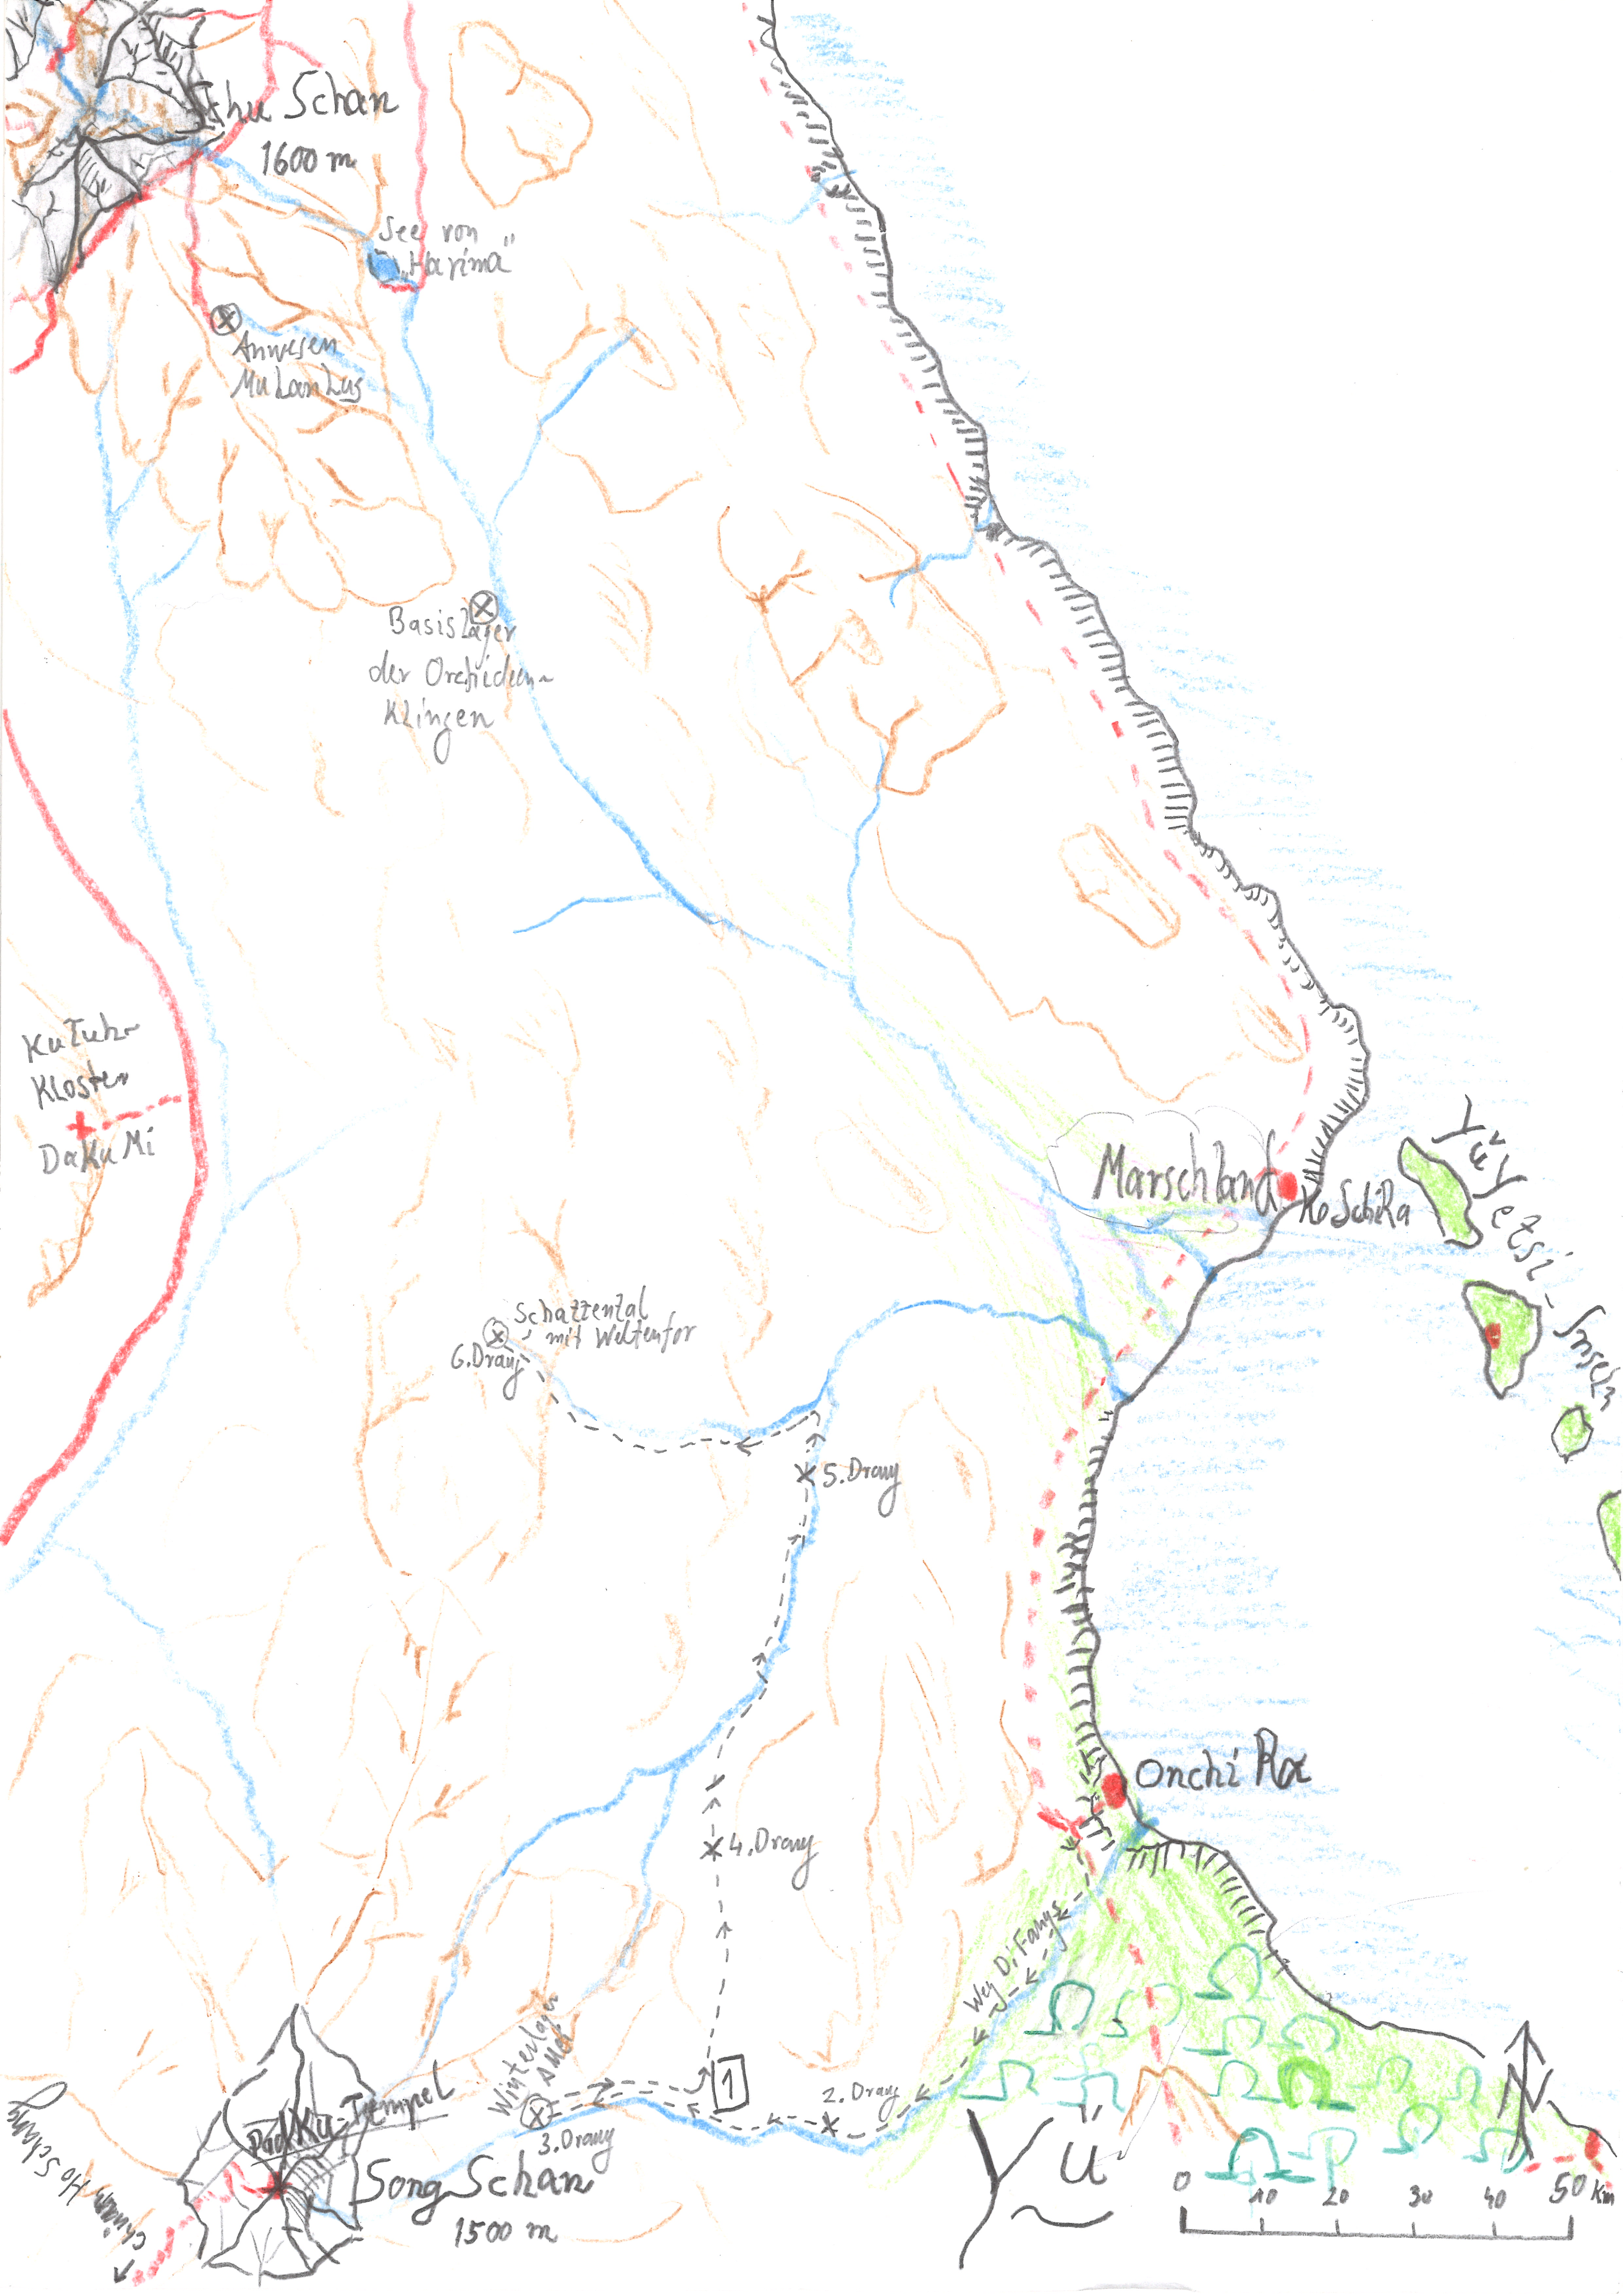
\includegraphics[width=17.5cm]{map.jpg}
  \caption{Die Provinz Yü}
  \label{fig:map-yue}
\end{figure*}

\section{Zwischen SchuSchan und SongSchan}
\label{yue}

Die Provinz Yü ist in [KTP\,101] kurz beschrieben.

Die Kartie in Abb. \ref{fig:map-yue} zeigt alle Orte an, die für das
Abenteuer relevant sind. Sie ist aber keineswegs vollständig. Es gibt
wesentlich mehr in der Provinz zu entdecken. Der SpL möge seinen
Ideenfluß in keinster Weise enschränken.

Die Siedlungsgebiet der Yü wird im Westen durch die Straße nach
ChüanHoSchang und im Osten durch das Meer begrenzt, wobei die
Küstendörfer nicht durch Yü bewohnt sind und auch nicht den
entsprechenden Ausnahmeregeln unterstehen. Sie müssen z.\,B. durchaus
Opfer auf den Weg der Tausend schicken.

Im allgemeinen ist die Vegetation im Hügelland eher karg. Die Täler
sind grüner, mit mitunter recht dichtem Buschwerk bis hin zu
regelrechten Wäldchen, vorwiegend Bambus. In Küstennähe südlich von
OnchiRa geht das Hügelland langsam in dichteren Wald und schließlich
in den Dschungel von Minangpahit über.

Das Wetter kann nach [KOM\,124] ermittelt werden (\emph{3E:
  Sommerfeuchte Zone}). Vor allem in den höheren Lagen des Hügellandes
kann es in den Winternächten empfindlich kalt werden mit regelmäßigem
Bodenfrost, der ab und an stark genug ist, um die Hügelkuppen mit
hübsch in der Morgensonne glitzerndem Reif zu überziehen. Zu
Niederschlägen kommt es um diese Jahreszeit fast nie. Dafür weht fast
immer ein starker Wind vorwiegend aus westlicher Richtung.

Die Yü kennen ihr Land sehr gut und bereisen es zu Fuß vergleichsweise
schnell unter Ausnutzung natürlicher Begebenheiten wie Wildwechsel und
Flußverläufe. Für sie hat das Gelände \textbf{Typ II}
[DFR\,85]. Ortsunkundige kommen durch die unwegsame Landschaft viel
langsamer voran, wenn sie einfach versuchen, möglichst schnell in eine
bestimmte Himmelsrichtung voranzukommen \textbf{(Geländetyp III)}. Wer
allerdings sich spurenlesend an die Fersen eines Yü heftet, kommt
natürlich auch in Genuß von dessen Ortskenntnis.

Neben der offensichtlichen Erwerbsquelle des Ginsenghandels spielt
auch die Ziegenhaltung eine große Rolle. Überall im Hügelland wird
man auf Ziegenherden stoßen.

Im folgenden werden besondere Orte von Nord nach Süd beschrieben,
gefolgt von einer Liste möglicher Begegnungen.

\subsection{See von Harima}

Soll das Abenteuer \emph{Das Schlemmermahl} [MSS\,5ff] nach KuroKegaTi
verlegt werden, bietet es sich an, den See von Harima hier an die
Hänge des SchuSchan zu versetzen.

\subsection{MuLanLuns Anwesen}
\label{mulanlus-anwesen}

MuLanLuns großzügig angelegter Landsitz befindet sich recht abgelegen
an den südlichen Hängen des SchuSchan, in einiger Entfernung von den
üblichen Lagen für die Anwesen der Reichen und Mächtigen aus KuenKung
und anderswo. Dies prädestiniert es als "`Krankenstation"' für das
Basislager der Orchideenklingen 50km südöstlich. Regimetreue
Immobilienbesitzer am SchuSchan lassen ihre Anwesen von OrcaMurai
bewachen. Die eher auf Unabhängigkeit bedachten bevorzugen ihre
eigenen, menschlichen Wachleute. Zu letzteren gehört natürlich auch
MuLan. Unbemerktes Eindringen in MuLans Anwesen ist nicht
einfach. Vielleich gelangen die SpF aber auch als Freunde hierher --
möglicherweise gar als Verwundete, wenn sie auf Seiten der
Orchideenklingen an einem Kampf teilgenommen haben.

Zu Beginn des Abenteuers befinden sich drei Orchideenklingen in
Behandlung. Zwei Kämpfer sind bereits verstorben und wurden mangels
Alternative diskret auf der Familiengrabstätte der Lun bestattet. Die
frischen Gräber sind noch deutlich sichtbar. Während des Abenteuers
werden immer wieder Verwundete und Gefallene eingeliefert.

Gerade an diesem Ort erscheint die ganze Unternehmung besonders brutal
und sinnlos. MuLan wird immer skeptischer und diskutiert die Sinnfrage
ganz offen mit den Orchideenklingen, möglicherweise gar mit LonChen
selbst, sollte er das Anwesen besuchen.

\subsection{Basislager der Orchideenklingen}

Vom gut in einem kleinen Nebental verborgenen Basislager aus führen
die Orchideenklingen ihre Operationen aus. Ab und an gibt es einen
koordinierten Angriff auf einen Handelszug der Xuan. Die meiste Zeit
patroullieren kleinere Gruppen durch Yü, um Ginsengsammler zu bekehren
und Informationen über bevorstehende Aktivitäten der Xuan zu
sammeln. So kam es auch dazu, daß KokoRo ausgesendet wurde, um DiFang
auf die eigene Seite zu ziehen oder hinter sein Geheimnis zu kommen.

Ein langjähriger Assistens MuLans versorgt die im Lager eintreffenden
Verwundeten und schickt die schwereren Fälle zu MuLans Anwesen.

Die SpF werden das Basislager kaum zufällig entdecken, aber sie
könnten als Gefangene oder Verbündete hierhin gebracht werden (im
Zweifelsfalle mit verbundenen Augen).

\subsection{Kloster DaKuMi}

Zwei Wegstunden westlich der Straße nach ChüanHoSchang, an den
ansteigenden Hängen des westlichen Teils der Neun-Blumen-Berge, gehen
im Kloster DaKuMi die Mönche des KuTuh ihrem unaussprechlichem Tun
nach. MiTo, der Abt, ist Mitglied der Familie Xuan und hat das Kloster
den SaMurai seiner Familie als Basislager zur Verfügung gestellt. Dies
ist in vielerlei Hinsicht das genaue Gegenstück zum Basislager der
Orchideenklingen. LiXuan sucht das Kloster häufiger auf, um die
Aktionen seiner SaMurai und Händler zu koordinieren.

Die Werte MiTos finden sich in [DSH\,101], wobei der acht Jahr jüngere
MiTo natürlich noch auf einem geringeren Grad steht und über weniger
Fähigkeiten verfügt. Wahrscheinlich wird dies für das Abenteuer aber
irrelevant sein.

\subsection{KoSchiRa}

Ähnlich wie OnchiRa ist KoSchiRa ein einfaches Fischerdorf. Allerdings
besteht das ganze Dorf aus fanatischen KuTuh-Anhängern, die hier --~so
verbunden mit seinem Element und so fern der institutionalisierten
Verehrung in den zivilisierteren Teilen des Reiches~-- ganz eigene,
besonders schreckliche Formen der Anbetung ihres dämonischen Gottes
entwickelt haben. Unsägliche Rituale finden am Meer und in den nahen
Sümpfen statt, als deren Folge sich sogar das Aussehen der
Dorfbewohner verändert hat. Sollte es die SpF wirklich hierher
verschlagen, kann der SpL hemmungslos Anleihen bei H.\,P. Lovecraft
nehmen, um eine passende Stimmung zu erzeugen. (Hier drängt sich vor
allem \emph{Schatten über Innsmouth} als Beispiel auf, wohlgemerkt
lediglich als Inspiration für die Stimmung. Die Handlungsdetails
passen selbstverständlich nicht. Bislang wurden auf Migard noch keine
Tiefen Wesen gesichtet\dots)

\subsection{Das Marschland}

Zahlreiche der Bäche und Flüßchen, die die östlichen Neun-Blumen-Berge
durchziehen, münden hier in einem ausgedehnten Delta ins Meer. Während
gerade im Winter viele Bäche austrocknen, ist das Delta ganzjährig
wasserführend. Bei Flut drückt das Meer Salzwasser ins Delta. Die
Landschaft ist von Salzsümpfen und Marschland geprägt. Die
Küstenstraße führt auf Knüppeldämmen über die sumpfigen Stellen, wird
aber schlecht unterhalten und ist bei Hochwasser häufig überschwemmt.

Als ob die finsteren Kultstätten der Bewohner KoSchiRas noch nicht
genug wären, trifft man im Sumpf auf allerlei unangenehmer
Zeitgenossen. Der SpL darf alle Register des Bestiariums ziehen. Neben
normalen Blutegeln [BES\,362] gibt es sogar Todesegel [BES\,372].

\subsection{Das Schattental}

Am Ende eines schmalen verborgenen Tales, das DiFang
\emph{Schattental} getauft hat, befindet sich ein von den Arracht in
grauer Vorzeit errichtetes permanentes Weltentor nach RenSchenYo. Über
dieses Weltentor wurde der Ginseng nach Midgard importiert. Für die
Priester des Ginsenggottes ist dieser Ort ebenso heilig wie
verstörend. Daher haben sie am Eingang des Tales, das den einzigen
begehbaren Zugang zum Weltentor darstellt, in die dichte Vegetation
ein sogenanntes \emph{Tabu} geflochten. Es führt dazu, daß denkende
Wesen, die sich dem Tabu nähern, unbewußt von ihm wegsteuern. Dadurch
wurde das Tal unauffindbar. Wer hingegen schon genau weiß, wo das Tal
ist, und bewußt in das Tal hineingehen will, dem gelingt das ohne
Probleme. Wesen mit tierischer Intelligenz sind vom Tabu nicht
betroffen. Die düstere Ausstrahlung der uralten Gebäude rund um das
Weltentor sorgt aber dafür, daß sich nur selten ein Tier ins Weltentor
verirrt (und selbst dann wird es von den Hunar wieder nach Midgard
geschickt, siehe Abschnitt \ref{hunar}). DiFang hat das Tal durch
einen Zufall entdeckt. Eine seiner Ziegen wurde durch ein Raubtier
verletzt und floh panisch in die dichte Vegetation am Eingang des
Tales. DiFang folgte ihrer blutigen Spur und umging so den Zwang des
Tabus. Die Xuan-SaMurai, die DiFang verfolgt haben, sowie die
Orchideenklingen, die wiederum die SaMurai verfolgt haben, wurden
ebenfalls durch äußere Einflüsse, nämlich die verfolgten
Spuren. Genauso können die SpF durch das Verfolgen der Spuren ins Tal
gelangen. Eine andere Möglichkeit wäre, den mitunter auftretenden
Luftrochen auf ihrem Heimweg zu folgen (siehe Abschnitt
\ref{begegnung-luftrochen}), wobei sie hierbei möglicherweise den
Talkessel aus einer unzugänglichen Richtung entdecken. Selbst dann
kann aber eine systematische Suche nach einem Zugang in den nun
bekannten Talkessel die ablenkende Kraft des Tabus überwinden.

\subsubsection{Der Ort des Tabus}

Direkt am Eingang zum engen und von den Seiten unzugänglichen
Schattental befindet sich das Tabu. Es ist ins Erdreich und in die
hier sehr dichte Vegetation eingewoben und manifestiert sich durch
auffällige spiralartige Muster, in der die Pflanzen und Bäume,
darunter auch etliche Ginsengpflanzen (\textbf{EW:Pflanzenkunde}), in
einem Umkreis von 3m wachsen. Der Ort hat eine starke Dweomeraura.

Der Ginsenggott der Yü ähnelt eher einem Ginseng-Totemgeist. Die
Priester des Ginsengkultes zählen spieltechnisch als Schamanen. Das
Tabu ist für sie ein heiliger Ort [ARK\,61], allerdings ist die
Kenntnis von seiner Lage in Vergessenheit geraten -- und die
ablenkende Wirkung des Tabus wirkt auch auf die Priester des
Ginsenggottes selbst. Durch sorgfältiges Vernichten aller Vegetation
am Ort des Tabus, inklusive des unterirdischen Teils, könnte man das
Tabu aufheben (und würde sich dabei natürlich den immerwährenden Zorns
des Ginsenggottes zuziehen). Austreiben oder Bannen der Wirkung ist
nicht möglich, da es sich um Dweomer handelt.

Etwa 30m weiter ins Tal hinein liegen die Leichen zweier Krieger mit
dem Dreizackinsignien der Xuan. Waffen und Wertgegenstände wurden
ihnen abgenommen. Auffällig an ihrem Marschgepäck ist ansonsten noch
ein kleiner Käfig mit zwei erstochenen Tauben. Dies sind Brieftauben
zur Kommunikation mit den Xuan in KuenKung, die die Orchideenklingen
wohlweislich getötet haben. Die beiden haben Schnittwunden am
Hals. Eine genauere Untersuchung bringt an den Tag, daß einer der
beiden ein gebrochenes Bein und eine Stichwunde ins Herz aufweist. Mit
einem \textbf{EW:Erste Hilfe} läßt sich feststellen, daß die
Schnittwunden von RengKwan (Wurfringe) stammen. Einer der beiden wurde
an der Halsschlagader getroffen und ist verblutet, während der andere
wohl erst im Nahkampf erledigt wurde. Auch der Zeitpunktes des Kampfes
kann geschätzt werden. (\emph{Heilkunde} kann wie üblich für
\textbf{WM+4} auf den Wurf für \emph{Erste Hilfe} eingesetzt werden.)
Ein \textbf{EW:Spurenlesen} verrät, daß hier 5--8 Personen gekämpft
haben. Ein Teil von ihnen hat sich von den üppig mit Vegetation
bewachsenen Hängen am Rand des Tals auf die Opfer gestürzt. Hat der
\textbf{EW:Spurenlesen} mindestens 24 erreicht, findet die SpF sogar
heraus, daß eine einzelne Figur den Hang hinauf geflohen ist. Dort
läßt die Vegetation allerdings bald nach. Eine weitere Verfolgung der
Spur auf dem nackten Fels ist beim Alter der Spur ohne Aussicht auf
Erfolg. Nach dem blutigen Kampf sind 3--4 Personen weiter ins Tal
gelaufen.

Was ist nun wirklich geschehen? Als DiFang am 6. Draug das Tabu hinter
sich gebracht hatte und einige Meter ins Schattental gelaufen war,
hielt er wie üblich kurz inne. Er wußte, daß hierher ihm nie jemand
folgen konnte. Diese Gewißheit war wie immer Balsam für seine
Einsiedlerseele. Und so ließ er sich ins hohe Gras nieder und ruhte
sich aus. Dies bekamen die SaMurai nicht gleich mit, und so näherten
sie sich mehr als beabsichtigt. DiFang, der die Ruhe des Tales genoß,
wurde nun endlich auf seine Verfolger aufmerksam und stellte sie
erschrocken zur Rede. Die bedrängten ihn mit gezogenen Waffen und
forderten ihn auf, sich zu ergeben und sein Geheimnis
preiszugeben. Während sich all dies ereignete, schritten wiederum die
Orchideenklingen zur Tat, die die dichte Vegetation zum Anlaß genommen
hatten, sich besonders nah an die SaMurai heranzuschleichen. Sie
kletterten an einer hier noch recht zugängliche Talwand hinauf und
näherten sich so den drei Kriegern unauffällig von der Seite. Aus dem
Hinterhalt warfen sie ihre Wurfringe. Der erste ging am Hals getroffen
zu Boden, der zweite floh über die gegenüberliegende Talwand, und den
dritten erledigten sie im Nahkampf (mit KanaUchi das Bein gebrochen
und den Wehrlosen dann erstochen, wobei der SaMurai einer der
Orchideenklingen noch eine üble Beinverletzung zufügen konnte). DiFang
sah das alles entsetzt an. Als die maskierten Orchideenklingen auf ihn
zukamen, geriet er in Panik. Statt seinen Rettern zu danken, lief er
ins Tal hinein, und die Orchideenklingen hinterher.

Das einer der SaMurai leichtfüßig entkommen konnte, kann nach Ermessen
des SpL noch ein Nachspiel haben. Der Entflohene läuft nämlich
schnurstracks zum Kloster DaKuMi, um Verstärkung zu holen. So er es
denn schafft, sich genau genug an den Weg zu erinnern, um das Tabu
wieder zu überwinden (keine Selbstverständlichkeit unter den gegebenen
nicht gerade streßfreien Umständen), kann die Verstärkung (in vom SpL
zu bestimmender Stärke) frühestens am 12. Draug im Schattental
eintreffen. Der SpL kann hier einer kampfversessenen Gruppe eine Show
bieten.

\begin{figure*}[t]
  \centering
  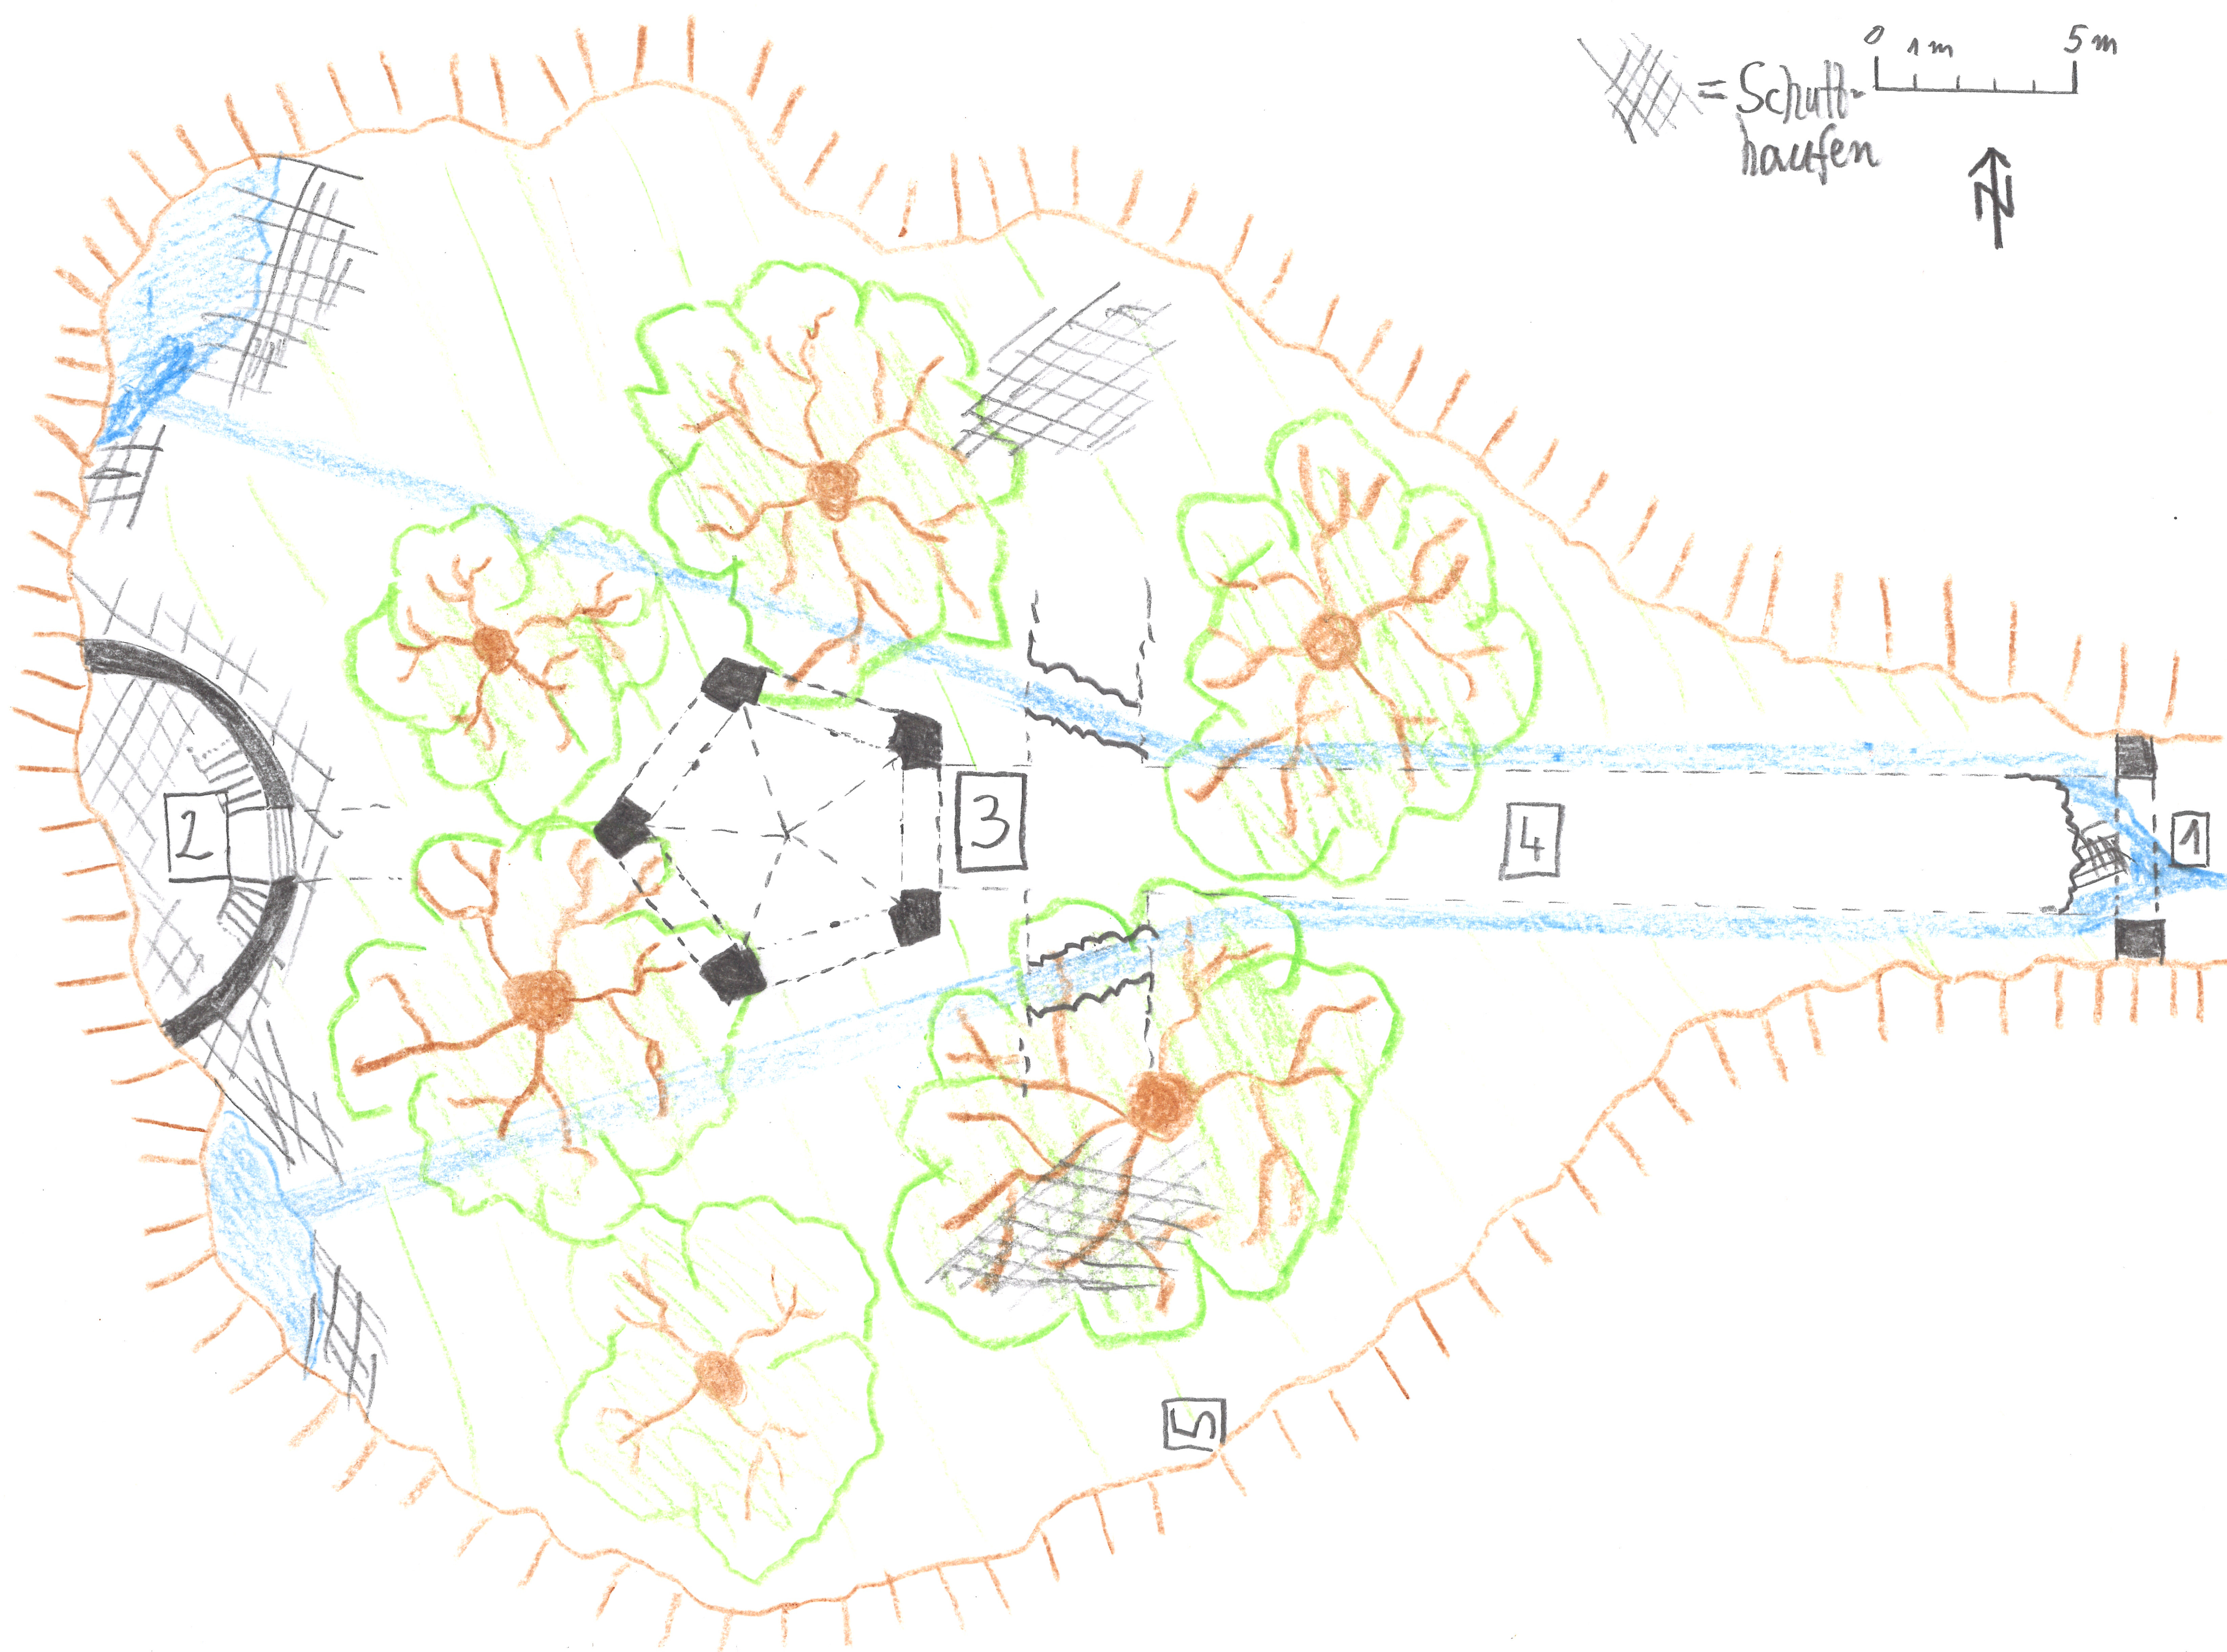
\includegraphics[width=17.5cm]{tor1.jpg}
  \caption{Die Midgard-Seite des Weltentores}
  \label{fig:tor1}
\end{figure*}

\subsubsection{Vorm verschlossenen Weltentor}

Eine Karte des Talkessels am Ende des Schattentals findet sich in
Abb.~\ref{fig:tor1}. Vom Eingang des Tals bis dorthin sind es 3km. Die
Steilwände sind etwa 30m hoch und nahezu senkrecht. Sie zu erklimmen
bedarf einer kleinen Klettertour ([DFR\,154f], die Wände haben
\emph{einige Ritzen}). Aufgrund der dichten Vegetation ist nur schwer
zu erahnen, was sich unten im Kessel befindet, wenn man von der oberen
Kante in den Kessel hinabschaut. Nachts erkennt man allerdings leicht
das geheimnissvolle Leuchten des Tores (normalerweise weißlich, aber
seit DiFang das Tor umgepolt hat, leuchtet es gelblich).

Die Anlage wurde von den Arracht zwar in grauer Vorzeit errichtet, war
aber vor "`nur"' gut 3000 Jahren noch in Benutzung. Erst dann zogen
sich die Arracht endgültig aus dieser Gegend zurück. Dennoch ist
mittlerweile natürlich fast alles zu Staub zerfallen und von
Vegetation überwuchert. Die erhaltenen Gebäudeüberreste sind aus einem
dunkelgrauen granitartigen Stein. Das Gebäude mit dem Weltentor (siehe
\fbox{3}) ist durch die ihm innewohnende Magie besser erhalten, aber
dennoch von Moosen und Flechten bedeckt. Vom ganzen Ort geht eine
undefinierbare düstere und unheimliche Ausstrahlung aus, die SpF mit
angeborenem Sechsten Sinn oder hohem Zaubertalent besonders
bemerken. Es singen keine Vögel und man trifft auf fast keine
Tiere. Geräusche werden vielfach von den Wänden des Talkessels
zurückgeworfen. Sonnenlicht fällt nur selten in den tief
eingeschnittenen Kessel. Kein Lüftchen regt sich\dots SpF, die
Dunkelheim [HdB\,47ff] bereist haben, fühlen sich an dessen
Architektur und Ausstrahlung erinnert.

In den Bäumen halten sich etwa ein halbes Dutzend Luftrochen auf, die
durch das z.\,Zt. "`falschrum"' gepolte Tor nach Midgard gelangt sind
und nun nicht mehr zurückkommen. Der SpL kann sie zu dramatisch
passenden Augenblicken ins Geschehen eingreifen lassen. Bei
Suchaktionen oder durch Kämpfe aufgeschreckte Luftrochen greifen
möglicherweise in Panik wahllos an. Wenn einzelne Figuren sich unter
den Bäumen herumtreiben, werden sie vielleicht als Beute
interessant. \emph{Sehen}, \emph{Hören} oder \emph{Wahrnehmung} hilft
bei der frühzeitigen Entdeckung durch die SpF.  Weitere Luftrochen
erkunden die Umgebung (vgl. Abschnitt
\ref{begegnung-luftrochen}). Bald nachdem das Tor wieder Richtung
RenSchenYo gepolt worden ist, fliegen die Luftrochen nach und nach
instinktgetrieben durch das Tor zurück nach RenSchenYo.

\textbf{\fbox{1} Portal}

\fbox{\pbox{0.96\linewidth}{%
Eine 8m hohe Mauer mit einem knapp 4m breiten und 6m hohen Rundbogen
überspannt das Tal. Das Mauerwerk aus einem dunkelgrauen granitartigen
Stein ist dicht mit Ranken überwuchert. Man erkennt noch mächtige
Angeln, in denen wohl mal Tore hingen. Ein aus dem Talkessel
fließendes Rinnsal hat sich tief in den Boden eingeschnitten.
}}

Ursprünglich wurde das Wasser unter der Straße entlanggeführt. Im
Laufe der Jahrtausende hat das Wasser die Kanalkonstruktion zum
Einsturz gebracht.

\textbf{\fbox{2} Eingestürzter Turm}

\fbox{\pbox{0.96\linewidth}{%
    Die Reste eines wuchtigen, an die Felswand gebauten
    Turmes. Lediglich die Mauern des Erdgeschosses ragen noch aus dem
    Schuttberg. Den Stumpf einer Wendeltreppe nach oben und eine
    weitere Wendeltreppe in den völlig verschütteten Keller kann man
    gerade noch erahnen.}}

Im Turm gibt es auch nach mühseliger Buddelei nichts zu finden. Hier
kampieren allerdings die vier Orchideenklingen.

Nachdem die Orchideenklingen den Kampf im Schattental beendet hatten,
redeten sie auf DiFang ein, um ihn von ihrer Sache zu überzeugen. Der
aber geriet in Panik und lief ins Schattental hinein. Die
Orchideenklingen natürlich hinterher. DiFang lief direkt ins Tor und
polte es sogleich von der anderen Seite um. Die Orchideenklingen
konnten den Farbwechsel von weiß auf gelb beobachten und mußten dann
feststellen, daß sie DiFang nicht folgen konnten. Sie schlugen
daraufhin ihr Lager im eingestürzten Turm auf. Von dort beobachten sie
seither das Tor und pflegen ihren schwer verwundeten Kameraden. Sie
sind stets wachsam und patroullieren gelegentlich durch den
Talkessel. SpF, die die Wände des Kessels herunterklettern, werden
automatisch bemerkt. Ob die Orchideenklingen sich dann allerdings
bemerkbar machen oder erstmal weiter die Lage beobachten, muß der SpL
situationsbedingt entscheiden.

Bei den Orchideenklingen handelt es sich um KokoRo, also um die unter
den OrcaMurais vermutete Schwester einer der SpF, und ihre Gefährten
Kai (m), Fu (m) und TanChi (w). Fu hat eine schwere Beinverletzung und
viel Blut verloren (am Ende des Kampfes hatte er noch 4LP und die
Verletzung \textbf{56--64} auf Tabelle 4.5 [DFR\,246] erlitten). Bei
der wenig professionellen Behandlung, die er z.\,Zt. genießt, wird er
sein Bein am 19. Draug wieder einsetzen können. Dies ist auch der
Zeitpunkt, wo sich die Orchideenklingen von sich aus auf den Weg
zurück ins Basislager machen.

Die Interaktion zwischen Orchideenklingen und SpF kann sich ganz
unterschiedlich entwickeln. Die Orchideenklingen sind naturgemäß
extrem mißtrauisch und halten die SpF erstmal für Spione der Xuan,
zudem sie ja damit rechnen müssen, daß der entflohene Xuan-SaMurai
Verstärkung holt. Wenn die SpF ihrem verletzten Kameraden helfen
können, wäre das ein willkommener Anlaß, das Mißtrauen
abzubauen. Außerdem besteht jederzeit die Chance, daß KokoRo ihre
Schwester bzw. ihren Bruder wiedererkennt. Andersrum kann dies nur
geschehen, wenn KokoRo ohne Maskierung auftritt. Der SpL hat es in der
Hand, das Timing hier möglichst spannend und dramatisch zu gestalten.

\textbf{\fbox{3} Weltentor}

\fbox{\pbox{0.96\linewidth}{%
    Ein fünfeckiges klobiges Gebäude mit 3,5m breiten und 5m hohen
    Torbögen auf jeder Seite, hinter denen nur ein neblig-gelbliches
    Leuchten zu erkennen ist. Das spitze Dach besteht aus fünf nicht
    besonders steil ansteigenden Steinflächen.}}

Dies ist das Weltentor nach RenSchenYo. Die Arracht haben es in grauer
Vorzeit errichtet. Nicht nur ist dieses Tor permanent und deutlich
größer als üblich, es wurde auch in ein magisch haltbar gemachtes
Steingebäude eingepaßt, so daß es nahezu unzerstörbar ist.

Normalerweise ist das Tor so gepolt, daß es in Richtung RenSchenYo
führt. Auf Midgard wagen sich wegen der düsteren Ausstrahlung des
Ortes nur wenige Tiere in die Nähe, und das Tabu verhindert die
Annäherung neugieriger intelligenter Wesen. Ist das Tor allerdings in
Richtung Midgard gepolt, passiert es schon häufiger, daß ein
Flugrochen aus Versehen durch das Tor fliegt. Daher sammeln sich nun,
wo DiFang das Tor nach seiner Flucht zur Abriegelung umgepolt hat,
Luftrochen in der Umgebung der Midgard-Seite des Tores.

Das Tor ist also z.\,Zt. von Midgard aus undurchlässig. Die Torbögen
fühlen sich an, als ob sie mit gelb leuchtendem Milchglas verschlossen
sind, daß sich natürlich nicht mit Gewalt überwinden
läßt. Glücklicherweise hat Ming aber den SpF das Schlüsselwort
"`Kra'anesch"' verraten. Sie müssen nur noch erkennen, daß sie sich
jetzt in der entsprechenden Situation befinden. Kra'anesch ist
übrigens der Name, den die Arracht RenSchenYo gegeben haben. Über die
Jahrtausende wurde durch Verballhornung aus Kra'anesch schließlich das
KanThaiTun-Wort \emph{RenSchen} -- also Ginseng. Daß DiFang die von
ihm wiederentdeckte Welt dan RenSchenYo, also in etwa
\emph{Ginsengwelt}, genannt hat, entbehrt nicht einer gewissen Ironie.

Das Tor läßt sich im Prinzip durch \emph{Bannen von Zauberwerk}
bannen. Allerdings muß das Zauberduell gegen \textbf{Zaubern+24}
gelingen, und \emph{Bannen von Zauberwerk} muß \textbf{fünfmal}
erfolgreich angewendet werden, bevor die magische Energie des Tores
genügend geschwächt worden ist.

Wenn die SpF ganz um das Gebäude herumgehen, werden sie auf jeden Fall
von den Orchideenklingen entdeckt. Ansonsten besteht eine
Wahrscheinlichkeit von 10\%\ pro 10min, daß eine patroullierende
Orchideenklinge sie am Weltentor bemerkt.

\textbf{\fbox{4} Straße}

\fbox{\pbox{0.96\linewidth}{%
    Eine erstaunlich wenig überwucherte Straße aus 1m mal 1m großen
    Steinplatten. Links und rechts der Straße fließt Wasser durch
    Gräben, die sich im Laufe der Zeit sehr tief in den Boden
    eingeschnitten haben. Die Straße erscheint dadurch geradezu aus
    dem Boden aufzuragen. Am Ende der Straße kann man noch Reste von
    einst nach links und rechts über den Graben führenden Brücken
    erkennen. Jenseits des Grabens verlieren sich die Straßenreste in
    überwucherten Schutthaufen.}}

Es braucht einen \textbf{EW-4:Spurenlesen}, um zu erkennen, daß die
Orchideenklingen hier am 6. Draug die Straße entlang und am Weltentor
vorbeigegangen sind. Gelingt ein weiterer \textbf{EW-4:Spurenlesen},
kann die Spur DiFangs identifiziert werden, der \emph{durchs} Tor
gegangen ist, d.\,h. seine Spur endet im geblichen Licht des östlichen
Torbogens. Machen die SpF hier laute Geräusche, werden die Orchideenklingen
bei \fbox{2} schon jetzt aufmerksam.

Die Kanäle speisen sich aus Quellen am westlichen Ende des Talkessels,
die dereinst kunstvoll zusammengeführt und in die Kanäle gelenkt
wurden. Jetzt haben sich durch die Schutthaufen kleine Seen gebildet.

\textbf{\fbox{5} Bambusütte}

\fbox{\pbox{0.96\linewidth}{%
Eine kleine einfach Bambushütte an die Felswand gebaut. Sie ist
offenbar bewohnt, enthält die einfachen Dinge des täglichen Lebens
eines Ginsengsammlers.}}

Dies ist DiFangs Hütte. Er zieht es vor, im abgeschiedenen Tal zu
leben, weil er als natürlicher Einzelgänger nicht gerne auf seine
Landsleute trifft. Ein \textbf{EW:Spurenlesen} führt zutage, daß es
hier \textbf{keine} frischen Spuren gibt und die Hütte wohl seit
etlichen Tagen nicht benutzt wurde. DiFang ist von hier am 26. Troll
aufgebrochen und seitdem nicht wiedergekehrt. (Bei seiner Rückkehr ins
Tal ist er ja auf der Flucht vor den Orchideenklingen direkt durchs
Weltentor gegangen.)

\textsc{Zukunft:} Die Bambushütte ist nach acht Jahren sichtlich
verfallen und offensichtlich unbewohnt.

\subsubsection{Ab durchs Tor!}

Um DiFang zu retten, muß sich mindestens eine SpF durchs Tor nach
RenSchenYo begeben. Da der eigentliche Sinn und Zweck des ganzen
Abenteuers ist, die SpF acht Jahre in die Zukunft zu transportieren,
muß es der SpL so arrangieren, daß irgendwann alle SpF sich auf
RenSchenYo aufhalten, und zwar lange genug, um das Vergehen von acht
Jahren auf Midgard zu rechtfertigen (was nicht sehr lange sein muß, da
es dem SpL obliegt, den aktuellen Unterschied im Verlauf der Zeit
zwischen Migard und RenSchenYo festzulegen). Tritt nicht der Idealfall
ein, daß eh alle SpF zusammen nach RenSchenYo gehen (bekannlich gilt
ja: \emph{Never split the party!}), dann hat der SpL verschiedene
Mittel an der Hand, dies zu handhaben. Zunächst einmal vergeht die
Zeit auf Midgard im Moment so viel langsamer, daß aus Sicht der auf
Midgard Zurückgebliebenen gewissermaßen nichts passiert. Selbst wenn
die durchs Tor gegangene SpF sich praktisch sofort entscheidet
umzukehren, dann werden auf Migard viele Stunden vergehen, bevor sie
wieder auftaucht. Der SpL kann die Spieler der Figuren, die sich auf
RenSchenYo aufhalten, in einen Nebenraum schicken und auch ab und an
scheinbar mit ihnen interagieren, einfach nur, um die restlichen
Spieler neugierig zu machen, was da nun passiert. Eine andere
Motivation, durchs Tor zu gehen, könnte die gleiche sein wie bei
DiFang: Flucht. Kommt es zum Konflikt mit den Orchideenklingen, zum
Angriff der Luftrochen oder gar zum Aufmarsch der Verstärkung der
Xuan-SaMurai, kann der Schritt durchs Tor ein eleganter Ausweg aus der
Situation sein. Bei friedlicher Interaktion mit den Orchideenklingen
könnte KokoRo darauf drängen, durchs Tor zu gehen, um DiFang zu finden
-- natürlich nur mit ihrem Geschwister und dessen Gefährten. Oder sie
stellt sich zur Verfügung, auf Midgard zurückzubleiben, um
irgendwelche Rettungsaktionen in die Wege zu leiten, die sich die SpF
wünschen mögen, falls sie nicht in einer gewissen Zeit
zurückkommen. Die anderen Orchideenklingen sind nicht besonders
gewillt, durchs Tor zu treten, und würden dies nur unter besonderen
Umständen tun.

Sobald die SpF durchs Tor getreten sind, stellt sich die Frage, ob
ihnen klar ist, daß sie das Tor auch ein weiteres Mal umpolen
können. Im Notfall hilft hoffentlich ein \textbf{Geistesblitz}. Polen
sie das Tor gewollt oder ungewollt nicht wieder um, können ihnen
natürlich weitere Personen von Midgard folgen. Hierbei ist zu
beachten, daß aus RenSchenYo-Perspektive alles auf Midgard ungeheuer
schnell passiert. Verfolger kommen also fast unmittelbar nach ihnen
durch das Tor. Gerade wenn die SpF vor den Xuan-Kriegern geflohen
sind, ist das eine realistische Option. Allerdings stellt sich die
Frage, ob die Krieger sich trauen, den SpF durch das Tor zu
folgen. Der SpL möge dies aufgrund der Kampfkraft der Gruppe und der
gewünschten Dramatik entscheiden. Immerhin bestehen auf RenSchenYo
Chancen, daß sich die Bewohner dieser Welt in einen eventuellen Kampf
einschalten -- hoffentlich zu Gunsten der SpF\dots\ Von den
Orchideenklingen wird ohne zwingende Gründe nur KokoRo das Tor
benutzen -- und das auch nur, wenn es dem SpL in den Kram paßt.

\subsection{OnchiRa}

Siehe Abschnitt \ref{biest} und [DSH\,34ff].

\subsection{AMeis Winterlager}
\label{winterlager}

AMei, die Älteste der Yü, hat weit im Süden, unweit des SongSchan, mit
ihrem weiteren Familienkreis und Gefolge ihr Winterlager
aufgeschlagen. Am 3. Draug ist DiFang hier eingetroffen, um AMei
Bericht zu erstatten, daß er sich entschlossen hat, sich ihrem Rat zu
beugen und nur noch mit den Xuan zu handeln. Bei dieser Gelegenheit
wollte er auch gleich die genauen Konditionen aushandeln (die durchaus
fair sind -- dem KuraiAnat geht es schließlich in erster Linie nicht
darum, Geld zu sparen, sondern sich selbst die Versorgung mit Ginseng
zu sichern und sie gleichzeitig ihren Gegnern zu verweigern).

Sollten die SpF im Lager auftauchen, können sie das Leben einer
größeren Gruppe Yü in ihren rasch erbauten Bambushütten
beobachten. Der kurze Besuch von DiFang ist kein Geheimnis, und man
gibt den SpF gerne Auskunft darüber. Wenn es um die Verabredungen mit
den Xuan geht, werden die Yü wortkarg und verweisen an AMei, die
selbst nur schwer zu einer Audienz zu bewegen ist und sich dann
ebenfalls recht verschlossen gibt.

Wenn der SpL will, kann er bei dieser Gelegenheit auch TsueChen
auftauchen lassen. Über das Tor im PadKu-Tempel auf dem Gipfel des
SongSchan [KTP\,101] kann er kurzfristig hier auftauchen, ohne zu
lange seine Aufgaben in KueiLi oder YenXuLu zu vernachlässigen. LiXuan
hatte ihn um diesen Besuch gebeten, um bei den Yü eindringlich
klarzumachen, daß die Staatsgewalt auch wirklich hinter den Xuan
steht. TsueChen ist überhaupt nicht erfreut, hier von Fremden gesehen
zu werden, und wird dies daher tunlichst vermeiden. Vielleicht
erhaschen die SpF aber doch einen Blick? Oder einige Yü, die die
schwarzgewandete Gestalt mit Knochenmaske mit seiner Leibgarde aus
zwei OgraMurai gesehen haben, berichten den SpF\dots

\textbf{2 OgraMurai} (Menschenähnliche, Gr4)\hfill In:\,m30\\
18\,LP, 30\,AP -- PR -- St\,100, Gw\,15, B\,16 -- MW\,22, EP\,6\\
\textsc{Angriff:} Stielhammer+7 (2W6+4), Faust+8 (1W6), Raufen+7 (1W6)
-- \textsc{Abwehr}+12,
\textsc{Resistenz}+12/14/12\\
\textbf{Bes.:} spurtstark, Infrarotsicht, --1 auf alle EW, WW und
Schadenswürfe bei Tageslicht

\subsection{PadKu-Tempel auf dem SongSchan}

Siehe [KTP\,101]. Wie schon erwähnt, bietet das Tor auf dem Gipfel
eine Möglichkeit, TsueChen oder ggf. auch LiXuan (der dann auch das
Tor nach YenXuLu im Tempel der Düsternis in KuenKung benutzen könnte)
hier kurzfristig auftauchen zu lassen, im Zweifelsfalle natürlich mit
Verstärkung durch OrcaMurai oder SaMurai der Xuan.

\subsection{Begegnungen}

Vorschläge für Begegnungen in der Wildnis, die der SpL passend zum
dramatischen Verlauf einflechten kann:

\subsubsection{Luftrochen}
\label{begegnung-luftrochen}

Luftrochen, die sich durch das seit dem 6. Draug umgepolte Tor nach
Midgard verirrt haben, schwirren nun auf Beutesuche durch die fremde
Welt. Die Wahrscheinlichkeit, auf sie zu treffen, ist je höher, je
näher man dem Weltentor kommt. Es obliegt dem SpL, die Angriffslust
der Luftrochen zu kalibrieren. Sie jagen einzeln und versuchen,
Kleingetier bis hin zu Ziegen zu erlegen -- was ihnen allenfalls
nachts gelingt. An eine schlafende SpF heranzuschweben mag ihnen als
lohnende Aktion erscheinen. Tagsüber kann man den dann recht hoch und
relativ langsam fliegenden Luftrochen eine ganze Zeit bequem
nachlaufen (solange bis ein Hindernis im Gelände das rasche
Vorankommen verhindert), um sich so nach und nach zum Weltentor führen
zu lassen.

\subsubsection{Tiger auf Ziegenjagd}

Ein Tiger hat sich aus dem nahen Dschungel Minangpahit nach Yü
begeben, um sich an Ziegen gütlich zu tun. Man trifft ihn daher am
ehesten im Süden an. Er ist nicht unbedingt auf einen Kampf mit
Menschen aus. Ein erlegter Tiger bringt allerdings das Wohlwollen der
Yü und von den Bewohnern OnchiRas mit sich, die über vagabundierende
Ziegenräuber nicht glücklich sind. Das Fell läßt sich für 250GS in
KuenKung verkaufen. Siehe [BES\,173f].

Werte siehe [BES\,173f].

\subsubsection{Yao in YamaOni-Gestalt}

Yao liebt Menschenfleisch, aber weil ihn sowas wie wahre Liebe zu
MeiHua gepackt hat, vermeidet er bei der Jagd die direkte Nähe
OnchiRas. Er liebt es, alleinreisende Menschen zu erlegen. Bei einer
größeren, gut gerüsteten Gruppe ist er klug genug, sich
zurückzuhalten. Einer Verfolgung kann er sich mit \emph{Beschleunigen}
relativ leicht entziehen. Dies ist dennoch eine Gelegenheit, Hinweise
zu sammeln. Vielleicht weisen Spuren Richtung Onchi Ra? Sollten die
SpF Yao zur Strecke bringen, ist ihnen der Dank der Yü, die schon
länger von Yao terrorisiert werden, sicher.

\subsubsection{Ginsengsammler der Yü}

Überall in der Provinz Yü kann man gelegentlich auf Angehörige des
Volkes der Yü treffen, die Ziegen hirten oder eben Heilkräuter und
Ginseng sammeln. Die Yü sind in der aktuellen Situation besonders
mißtrauisch gegenüber Fremden. Verschaffen sich die SpF aber das
Vertrauen oder den Respekt der Yü, können sie allen möglichen
Hügellandklatsch erfahren, wobei der SpL nach Belieben auch relevante
(wenn auch möglicherweise leicht verfälschte) Informationen über
DiFang und AMei, Xuan und Orchideenklingen, YamaOni und Luftrochen,
Schwarze Adepten und OgraMurai einmischen kann.

Einige Yü sind sehr gut im Spurenlesen. Möglicherweise können die SpF
so einen professionellen Spurenleser anheuern, um den Weg DiFangs
nachzuvollziehen.

Siehe auch [KTP\,131].

\textbf{Ginsengsammler der Yü} (Waldläufer, Gr1)\hfill In:\,m60\\
13\,LP, 8\,AP -- TR -- St\,65, Gw\,80, B\,26 -- MW\,16, EP\,2\\
\textsc{Angriff:} DaDao+7 (1W6+2), Bo-Stab+5 (1W6+1), Dolch+5 (1W6),
Raufen+7 (1W6--3) -- \textsc{Abwehr}+11,
\textsc{Resistenz}+10/12/10\\
\emph{Geländelauf+15, Kräuterkunde+5, Meditieren+8, Pflanzenkunde+5,
  Sprechen: KanThaiTun+14, Spurenlesen+6, Überleben im Wald+8,
  Wahrnehmung+4}

\subsubsection{Händler der Xuan}

Vorwiegend in der Nähe der Straße zwischen KuenKung und ChüanHoSchang
können die Spieler auf auf kleine Gruppen von Händlern der Xuan
treffen, die auf dem Weg zu Siedlungen der Yü sind oder von dort
kommen. Ginseng und andere Waren transportieren sie auf Kiang, also
eselartige Lasttiere. In der Regel haben sie als Wache ein paar
Samurai dabei. Genau wie die Yü sind sie in der gegebenen Situation
mißtrauisch und angespannt. Allerdings werden sie auch bei einer
freundlich verlaufenden Begegnung kaum Interna aus dem Hause Xuan
ausplaudern.

\textbf{Händler der Xuan} (Händler, Gr1)\hfill In:\,m60\\
11\,LP, 7\,AP -- LR -- St\,60, Gw\,60, B\,24 -- MW\,15, EP\,2\\
\textsc{Angriff:} Bo-Stab+7 (1W6+1), Dolch+5 (1W6), Wurfmesser+5
(1W6--1), Raufen+6 (1W6--3) -- \textsc{Abwehr}+11 (+13 mit Bo-Stab),
\textsc{Resistenz}+10/12/10\\
\emph{Gassenwissen+5, Geschäftstüchtigkeit+8, Geschenke machen+8,
  Kanthanische Schrift+12 (Schriftart 2), Menschenkenntnis+5,
  Schreiben: KanThaiTun+12, Sprechen: KanThaiTun+14, Wahrnehmung+4,
  Verhören+8}

\subsubsection{Überfall der Orchideenklingen}

Aus der Ferne können die SpF Zeugen werden, wie sechs Orchideenklingen
einen kleinen Handelszug aus drei Händlern und zwei Leibwachen mit
vier Kiang als Lasttiere überfallen. Die Orchideenklingen werfen
Wurfringe aus dem Hinterhalt und nehmen dabei auch Todesopfer in
Kauf. Gegner, die sich ergeben, werden aber nicht ermordet, sondern
lediglich gefesselt, um sie an der Verfolgung zu hindern. Nachdem sie
ihnen ihre Waren und Wertgegenstände abgenommen haben, überlassen sie
sie ihrem Schicksal.

\section{RenSchenYo -- die Ginsengwelt}

RenSchenYo ist eine kleine Urwelt aus der Spähre von Holz und Luft. Da
sie der Ordnung näher ist, vergeht die Zeit dort langsamer, im
langjährigen Durchschnitt etwa zehnmal langsamer. Eine Besonderheit
von RenSchenYo ist, daß diese Welt im arkanen Koordinatensystem
chaotisch oszilliert. Als die Arracht das Weltentor errichteten, war
sie Midgard besonders nahe, und die Zeit verging nur etwa halb so
langsam. Zur Zeit ist sie Midgard besonders fern (was aber der
Funktionstüchtigkeit des Weltentores keinen Abbruch tut). Den genauen
Faktor legt der SpL so fest, daß am Ende ihres Aufenthaltes die SpF
auch wirklich die gewünschten acht Jahre in die Zukunft gereist sein
werden. Dieser Faktor wird wohl sehr hoch sein, so daß fast alles auf
Midgard aus der Sicht RenSchenYos nahezu augenblicklich
passiert. Sollten also Verfolger sich nach einer Midgardstunde
entscheiden, ebenfalls durchs Weltentor zu schreiten, sind auf
RenSchenYo wohl nur wenige Sekunden vergangen.

Man beachte, daß auf RenSchenYo Zauber grundsätzlich \textbf{1\,AP}
mehr verbrauchen, während \textbf{Wundertaten} sogar \textbf{3\,AP}
mehr verbrauchen (siehe [MdS\,154]).

Der Himmel über RenSchenYo ist fast immer strahlend hellblau mit
gelegentlichen Schäfchenwolken, von erfrischenden Brisen
umhergetrieben. Die Sonne erscheint sehr hell, ist aber deutlich
kleiner als die Midgards. Sie geht in einem etwa zehnstündigen Rhytmus
auf und unter (nach Lokalzeit, versteht sich -- die SpF kommen zur
Mittagsstunde an). Nachts kann man das Phasenspiel von gleich vier
Monden beobachten. Das Klima ist regenwaldartig. Ähnlich erscheint die
überwältigende Flora und Fauna. Überall grünt und blüht und wuselt
es. Fast überall gibt es dichtes Buschwerk, aus dem nur gelegentlich
baumartige Strukturen emporwachsen. Das Unterholz geht gewissermaßen
direkt in den Boden über, der teils aus eng ineinandergewundenen Ästen
zu bestehen scheint, teils wie grob bröckelnder Torf daherkommt. Auf
Lichtungen und Wegen federt der Boden leicht unter den Füßen. Es gibt
insektenartiges Kleingetier, das aber weder unangenehm noch gefährlich
ist, und zahlreiche braun bepelzte Nagetiere, die die Hauptnahrung der
Luftrochen darstellen, die wohl noch am ehesten die Teile der Fauna
sind, mit denen die SpF sich auseinandersetzen müssen. Die häufigen
bunten Früchte sind in der Regel genießbar, aber das wissen die SpF
natürlich nicht. Jedem halbwegs pflanzenkundigen fällt allerdings auf,
daß überall sehr viele prächtig gedeihende Ginsengpflanzen anzutreffen
sind, mit wunderbar geformten saftigen Wurzeln. Investiert die Gruppe
4h in eine Suche und gelingt ein \textbf{EW:Pflanzenkunde} oder ein
\textbf{EW:Kräuterkunde}(bester in der Gruppe vorhandener Wert), kann
sie ein besonders prächtiges Exemplar finden, daß sie problemlos
mitnehmen können und mit den richtigen Verbindungen (z.\,B. über Ming)
in KuenKung für 2000GS verkaufen können. Ansonsten können sie
natürlich auch einfach wahllos Ginseng ernten, was für eine im
Reisegepäck noch gut mitzuführende Menge immer noch 500GS Erlös
bringt. Allerdings kann derartiges Raffen die Aufmerksamkeit und den
Zorn der Hunar erregen, siehe Abschnitt \ref{hunar}.

\begin{figure*}[t]
  \centering
  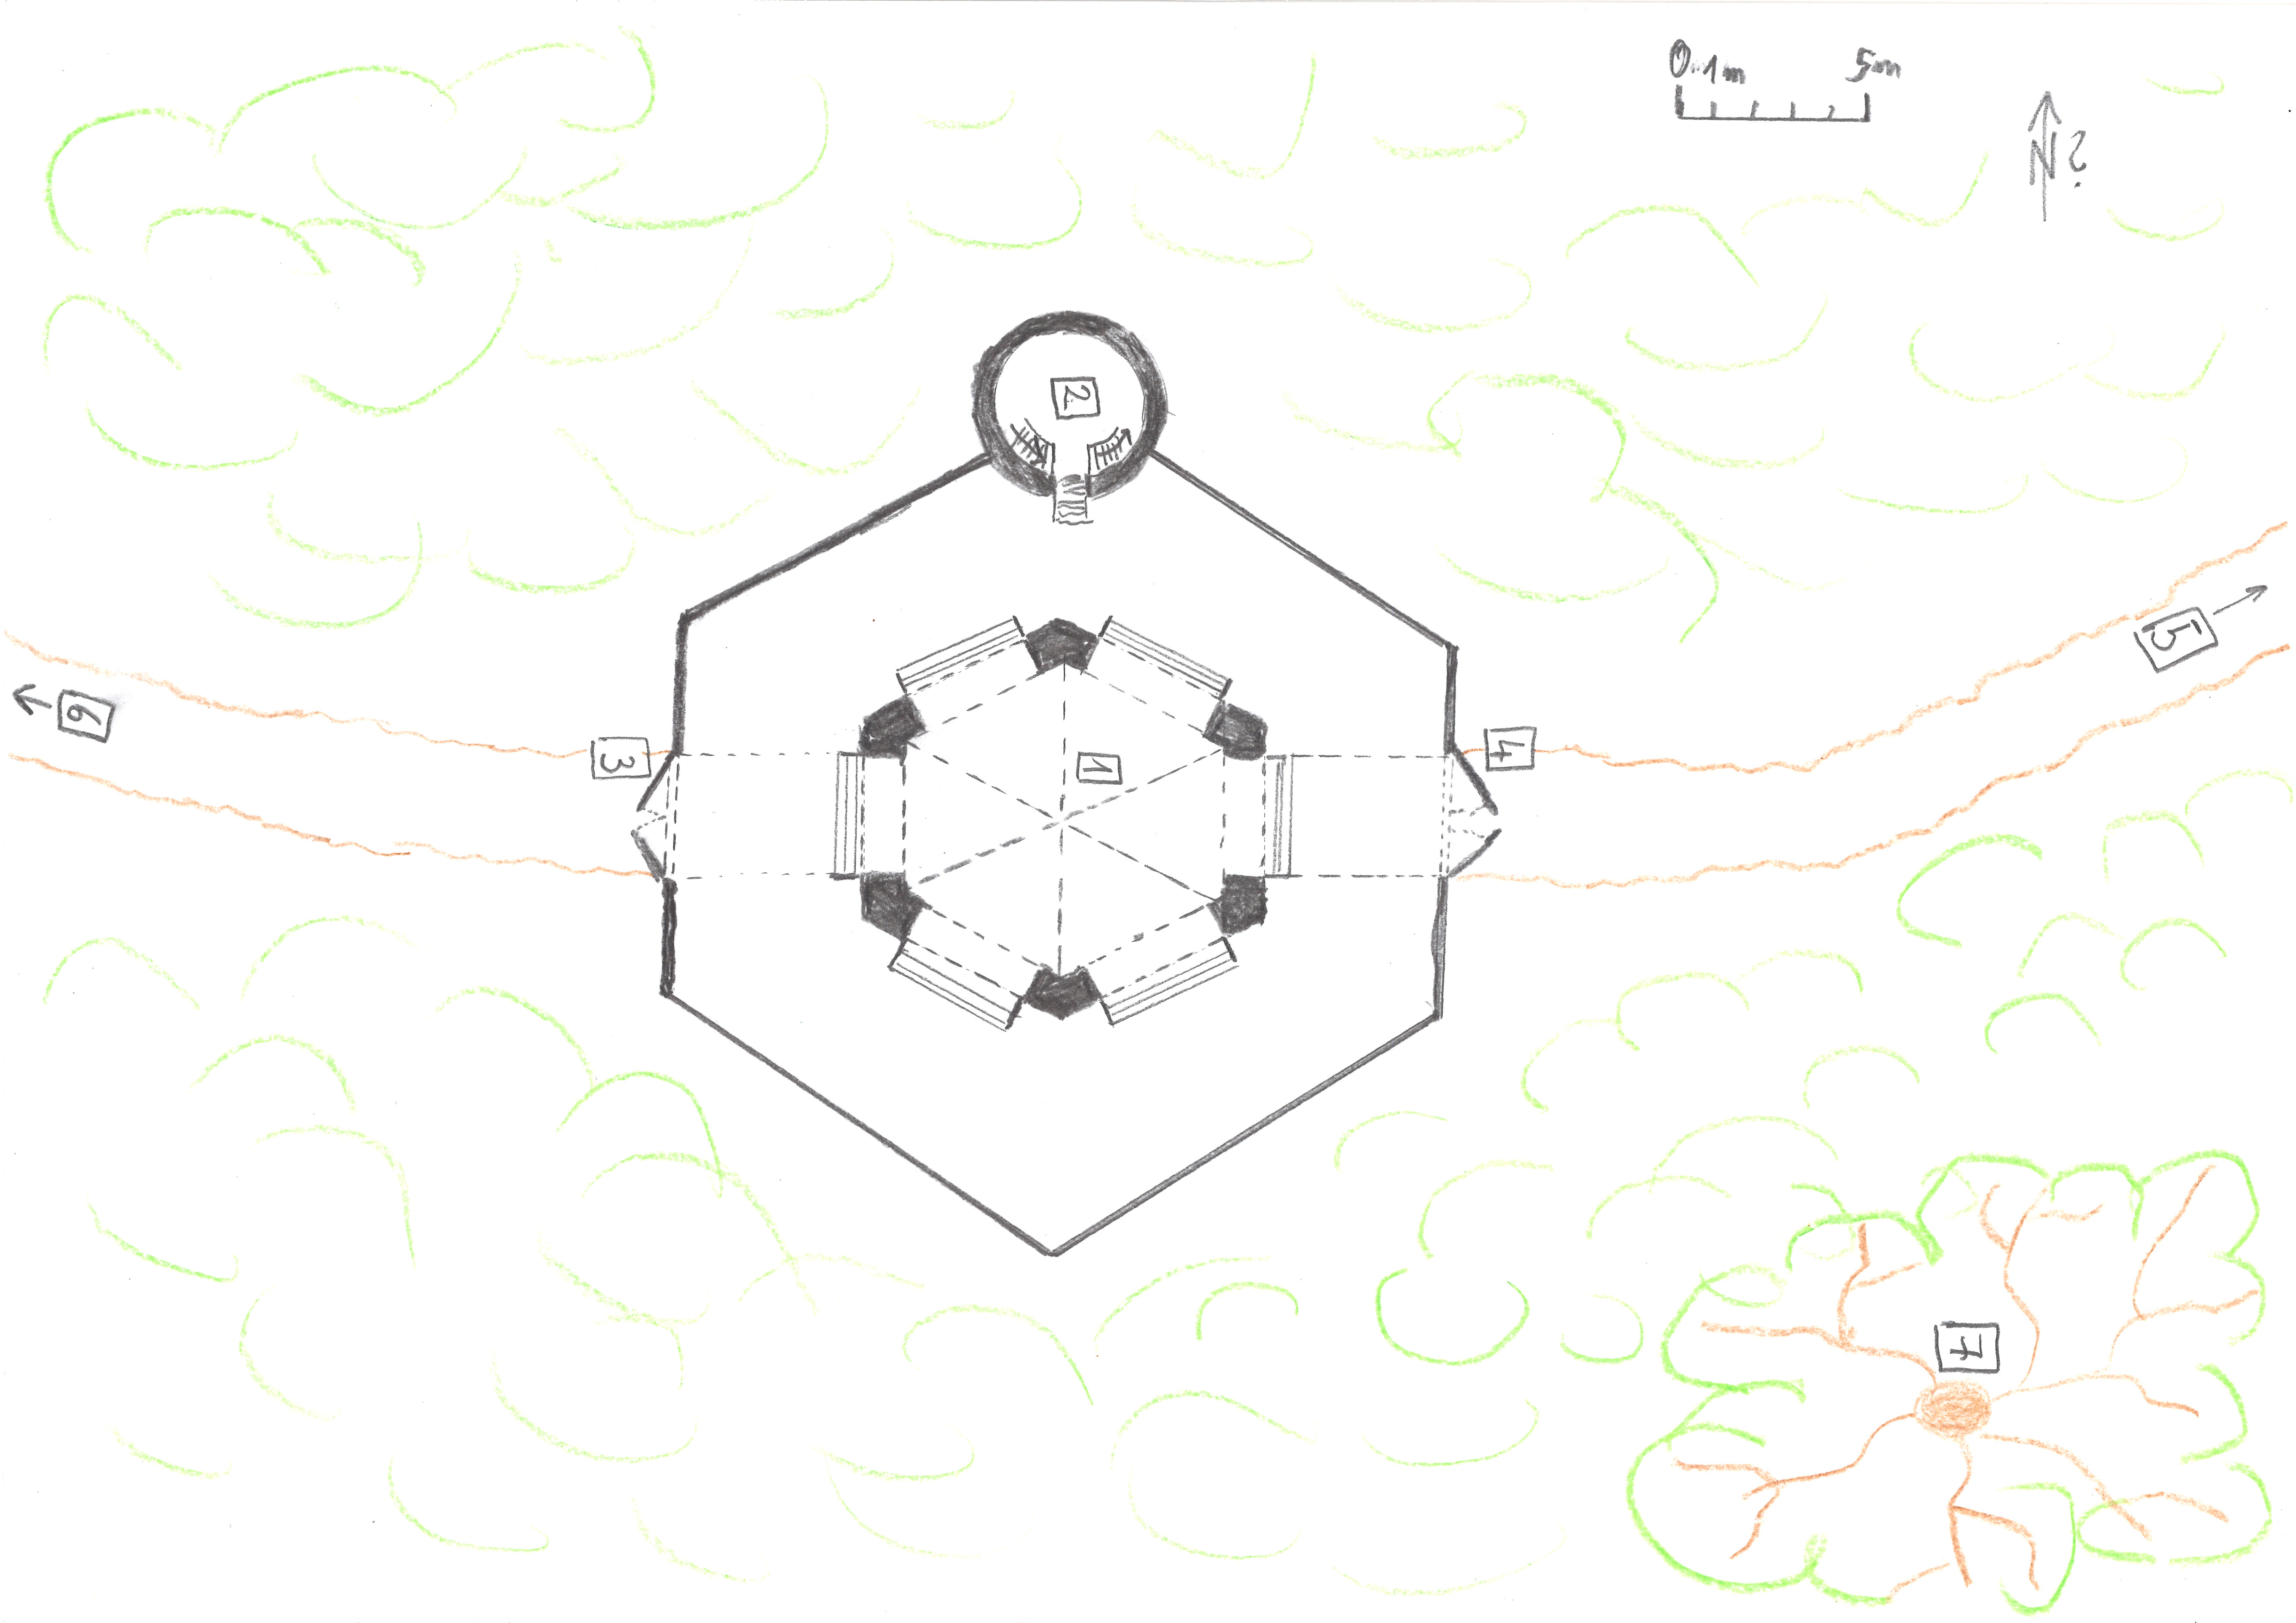
\includegraphics[width=17.5cm]{tor2.jpg}
  \caption{Die RenSchenYo-Seite des Weltentores}
  \label{fig:tor2}
\end{figure*}

\subsection{Die andere Seite des Tores}

Die Umgebung des Weltentores zeigt die Karte in
Abb.~\ref{fig:tor2}. Da seit Aufgabe der Anlage nur gut 300 Jahre
vergangen sind, sind die Gebäude hier wesentlich besser erhalten als
auf Midgard. Das aus Midgard mitgebrachte steinerne Baumaterial (der
gleiche dunkelgraue granitartige Stein) ist für die lokale Natur so
ungewohnt, daß selbst die gepflasterten Wege relativ wenig überwuchert
sind. Dennoch findet man überall zumindestens Moosflecken oder einen
efeuartigen Bewuchs.

\textbf{\fbox{1} Tor}

\fbox{\pbox{0.96\linewidth}{%
Das Torgebäude sieht ähnlich aus wie das auf Midgard, allerdings ist
es sechseckig und viel besser erhalten. Der umgebende gepflasterte
Platz ist auch nicht von Schutt oder Vegetation überdeckt, so daß man
noch die flachen Treppenstufen erkennen kann, die von jedem Torbogen
auf den Platz führen, und die elegante Wellen- und Spiralmuster im
Pflaster. Auch das Mauerwerk des Tores selbst läßt noch ähnliche
Verzierungen erahnen.
}}

\textbf{\fbox{2} Turm}

\fbox{\pbox{0.96\linewidth}{%
    Ein schlanker, etwa 20m hoher Turm, der Teil einer einfachen
    Befestigung rund um das Weltentor ist, die ansonsten aus einer 4m
    hohen Mauer besteht.}}

Die Wendeltreppe zur Rechten des Eingangs führt über mehrere Etagen
auf die Platform, von wo man sich einen guten Überblick über die
nähere Umgebung verschaffen kann (siehe Abschnitt
\ref{holzwolken}). Hinter einem lockeren Stein im zweiten Stock hat
DiFang seine ersparnisse versteckt: Jade, Geldschuhe und Edelsteine im
Wert von immerhin 6500GS.

Die Wendeltreppe zur Linken des Eingangs führt in den Keller und endet
an einer Metalltür, die sich mit einer aufaddierten Stärke von
100 relativ mühelos aufdrücken läßt. Allerdings ist sie mit einer
\textbf{Angstschwelle} gesichert (auf der Außenseite), siehe
[HdB\,52]. Das macht sich so bemerkbar, daß die Opfer hinter der Tür
größmögliches Grauen vermuten. Im Falle van KanThai z.\,B. eine Horde
OrcaMurais, unter denen sie ihre geopferten Verwandten vermuten. Je
weiter die Tür geöffnet wird, desto wilder drängen die Feinde dahinter
nach draußen\dots

Hat man die Angstschwelle überwunden, ist der Lohn der Mühe die Reste
des Aktenlagers der Arracht (zu deren Zutritt die Befugten mit
Schutzamuletten gegen die Angstschwelle ausgestattet waren). Unzählige
Papier- und Pergamentfetzen liegen auf dem Boden herum. Selbst wenn
man in der Lage ist, die Arrachtversalien zu entziffern, so wird man
nur langweilige Abrechnungen über Ginsenglieferungen und
Dorngleiterabrichtungen erkennen können. Wer sich allerdings
mindestens eine halbe Stunde Zeit nimmt, um das Zettelgewirr
sorgfältiger zu untersuchen, findet dann doch drei Spruchrollen,
\emph{Bannen von Zauberwerk}, \emph{Silberne Bannsphäre} und
\emph{Rauchwolke}, die den hier stationierten Arracht zur Verteidigung
dienten, dann aber im Chaos der Abreise irrtümlich zurückgelassen
worden sind.

\textbf{\fbox{3} Westtor}

\fbox{\pbox{0.96\linewidth}{%
Einst sicher sehr stattliche, nun aber verrostete metallene Torgitter
hängen noch halb in den Angeln. Ihre Ornamente spiegeln die Muster des
Platzes wieder.}}

Die Straße hinter dem Tor ist mit Steinplatten gepflastert. Sehr
zaghaft wagt sich die Natur wieder vor, so daß sich mittlerweile eine
Erdschicht mit etwas Pflanzenbewuchs gebildet hat.

\textbf{\fbox{4} Osttor}

\fbox{\pbox{0.96\linewidth}{%
Ein ähnliches Tor wie bei \fbox{3}.}}

Auch die Straße ist in einem ähnlichen Zustand wie bei \fbox{3}
beschrieben. Hier kann man allerdings mit einem
\textbf{EW+4:Spurenlesen} feststellen, daß vor kurzem ein Mensch
(nämlich DiFang) Richtung \fbox{5} gelaufen ist.

\textbf{\fbox{5} Weg zur Aussichtsplatform}

\fbox{\pbox{0.96\linewidth}{%
    Die Straße steigt leicht an und führt nach knapp 200m auf eine Art
    steinerne Aussichtsplatform. Von hier erkennt ihr, daß ihr euch
    offenbar auf einer Art Hochebene befindet, denn unmittelbar hinter
    der Brüstung der Platform fällt das Land zuerst mäßig und dann
    rasch steiler werdend ab. Man sieht keinen Talboden, sondern nur
    blaugrüne dunstige Weite, fast wie ein unter euch liegendes
    Wolkenmeer. In etwa 500m Enfernung sieht man eine benachbarte
    Hochebene aus dem Dunst aufsteigen.}}

Auf der Platform findet sich das bescheidene Reisegepäck DiFangs. Er
hat sich (auf der Zeitskala RenSchenYos erst vor wenigen Minuten)
frustriert auf die Platform geflüchtet, um hier, die Schönheit
"`seiner"' Welt beobachtend, über die Umstände nachzudenken. Dies hat
die zufällig in Gestalt eines Wirbelwindes in der Nähe weilende
BaiSseYuen angelockt, die DiFangs Kummer durch einen "`Streich"' das
Sahnehäubchen aufgesetzt hat: Sie hat den Armen einfach gepackt und
auf der nächsten "`Holzwolke"' abgesetzt. Siehe auch Abschnitt
\ref{holzwolken}. Aus DiFangs Sicht hat ihn ein Wirbelwind über den
Abgrund getragen -- nicht gerade ein Erlebnis, das zur geistigen
Stabilität beiträgt\dots.

Schaut man ein wenig in die Wolkenlandschaft, entdeckt man bald
diverse Luftrochen durch die Weite gleiten -- und ab und an auch einen
der größeren Dorngleiter.

\textbf{\fbox{6} Weg zur Abflugstelle}

\fbox{\pbox{0.96\linewidth}{%
    Nach 200m findet sich am Ende der leicht abfallenden Straße eine
    seltsame, halb verfallene Steinkonstruktion. Sie sieht aus wie
    sehr breite Stallungen, aber da, wo man die Pferde herausführen
    würde, gähnt ein bodenloser Abgrund.}}

Dies ist der "`Flughafen"' für die von den Arracht kontrollierten
Dorngleiter, der allerdings ebenfalls seit 300 Jahren nicht mehr
benutzt wird. Die Aussicht entspricht der bei der Aussichtsplatform
\fbox{5}. Auch hier kann man weitere der "`Holzwolken"' erkennen, hier
allerdings in etwas weiterer Entfernung.

\textbf{\fbox{7} Nest der Luftrochen}

\fbox{\pbox{0.96\linewidth}{%
Aus dem recht einförmig wenige Meter hohem Buschwerk ragt hier eine
baumartige Struktur 15m in die Höhe.}}

Solche Bäume gibt es auch noch häufiger, allerdings ist dies der dem
Tor nächste. Er dient einer Handvoll Luftrochen als Wohnstatt. Sollten
sich die SpF durch das Unterholz bis hierher vorkämpfen, werden sie
zur Belohnung von den Luftrochen unfreundlich empfangen.

\subsection{Hölzerne Wolken}
\label{holzwolken}

Nach und nach werden die SpF die Struktur RenSchenYos erahnen
können. Die vermeintlichen Hochebenen entpuppen sich als gigantische,
aus Holz gewachsene Strukturen, die wie Wolken in einer blaugrünen
Atmosphäre schweben. Man stelle sich das ähnlich vor wie die
Wolkenstadt bei \emph{Star Wars}. Die Holzwolken "`schwimmen"' alle
auf ähnlicher Höhe. Wer von einer Wolke herunterstürzt, fällt in die
dichter werdende bodenlose Atmosphäre, bis er durch steigenden Druck
und Temperaturen einen qualvollen Tod findet.

Die Wolke mit dem Weltentor ist mit etwa 500m Durchmesser ein eher
kleines Exemplar. Die Wolken bewegen sich langsam im Wind und kommen
sich auch manchmal auf einige hundert Meter nahe. Zusammenstöße gibt
es eher selten. Der größte Teil der Oberfläche RenSchenYos ist
"`wolkenlos"'. In manche Richtungen sieht man überhaupt keine
Nachbarwolke, oder nur ganz klein im Dunst viele Kilometer entfernt.

Die im Moment nur 500m entfernte nächste Wolke hat die Ehre, DiFang
beherbergen zu dürfen. Früher oder später sollten die SpF ihn (nach
einem \emph{Sehen}-Wurf o.ä.) dort erspähen können. Zu seiner Rettung
könnten sie sich um die Mithilfe eines der Bewohner RenSchenYos (siehe
nächste Abschnitte) bemühen. Die beiden Wolken kommen allerdings auch
langsam aufeinander zu, wie man nach längerer genauer Beobachtung
feststellen kann. Sie werden sich in einigen Tagen fast berühren. Mit
einem langen Seil (könnte mit etwas \emph{Seilkunst} auch aus Lianen
geflochten werden) kann man dann den Abgrund überbrücken. Je tiefer
man dafür wagt, den Abgrund hinunterzuklettern, desto kürzer ist die
zu überbrückende Strecke. Sollten die SpF diesen Weg gehen, hätten sie
eine sehr lange Zeit auf RenSchenYo verbracht. Zum Glück steuert ja
der SpL das Schicksal so, daß sie in jedem Falle acht Midgardjahre
später wieder nach Hause kommen. Dann ist die Zeit auf RenSchenYo eben
doch nicht ganz so langsam vergangen.

\subsection{Eine Weiße Wolke}

BaiSseYuen befindet sich nach ihrer Schandtat immer noch in der
Nähe. (Es sind ja wie gesagt bei Ankunft der SpF erst wenige Minuten
vergangen.) Sie hält sich zunächst verborgen und beobachtet
schadenfroh den Lauf der Dinge in Gestalt eines kaum sichtbaren
Wirbelwindes. Je nach dem, wie günstig der für DiFang und die SpF
ausfällte, kann sie sabotierend eingreifen oder aber auch
schlußendlich als Retter in der Not auftreten. Dazu wird es aber erst
nach komplizierten Verhandlungen kommen, in denen sie neckisch fragen
wird, was die SpF als Gegenleistung wohl für sie tun könnten. Guten
Vorschlägen ist sie durchaus aufgeschlossen. Die Freundschaft eines
Dschinns kann aber fatale Nebenwirkungen haben, vgl. das Schicksal
Mings in [DSH].

Durchaus möglich ist auch, daß BaiSseYuen zwischenzeitlich aus
RenSchenYo verschwindet und Ming hämisch Bericht erstattet vom
Schicksal seines Handelspartners und den kläglichen Rettungsversuchen
der von ihm beauftragten SpF.

\subsection{Zwei dicke Freunde}
\label{hunar}

Auf RenSchenYo lebt auch ein recht kurioses Paar: Zwei Hunar (siehe
[MdS\,249ff], ein Sturmriese (\emph{Gjornhune}) und ein Baumriese (in
KanThaiPan \emph{SchuDschuRen} genannt), sind \emph{best buddies} und
verstehen sich als sowas wie die Hüter dieser kleinen hübschen
Welt. Der Baumriese ist dabei fürs Grobe zuständig, während der
Sturmriese die Hauptaufgabe hat, seinen Freund von Wolke zu Wolke zu
tragen.

Auf DiFang sind die beiden durchaus schon aufmerksam geworden, aber da
er sich nie gierig gezeigt hat, verzeihen sie ihm die regelmäßige
Ginsengernte. Die beiden kennen das Schlüsselwort zum Umpolen des
Tores, und der Baumriese schickt auch die sich gelegentlich durchs Tor
nach RenSchenYo verirrten Tiere nach Midgard zurück.

Früher oder später wird die Gruppe auf die Hunar stoßen -- und dabei
hoffentlich nicht durch gieriges oder generell naturverachtendes
Verhalten ihren Zorn erregen. Die SpF können nicht mit den Hunar
sprechen. (Die bei Beschwörungen übliche Zwiesprache ist in dieser
Situation leider nicht möglich.) Aber mit Händen und Füßen wird
vielleicht eine Verständigung möglich sein. Es ist dem Sturmriese
natürlich ein leichtes, DiFang wieder von der Nachbarwolke
zurückzubringen, so man ihm erstmal klargemacht hat, worum es
geht. Auch muß DiFang überzeugt werden, bei der Sache mitzumachen,
denn er hat große Angst davor, schon wieder von einem Sturmwesen
gepackt zu werden. Schlußendlich könnte BaiSseYuen die Sache noch ein
wenig sabotieren.

In Ausnahmefällen nutzen die Hunar das Tor übrigens auch, um selbst
nach Midgard zu reisen. Vielleicht war dies der Weg, wie der
SchuDschuRen in die kanthanische Sagenwelt eingegangen ist\dots

Werte siehe [MdS\,249ff].

\subsection{Arracht}

Als vor etwa 3000 Jahren die Arracht auf Midgard immer mehr
zurückgedrängt wurden, kam die regelmäßige Nutzung des Weltentores zum
Erliegen. Einige der Arracht, die auf der Seite RenSchenYos
stationiert waren, beschlossen, auf dieser Welt, an deren Klima sie
angeaßt waren, zu verbleiben. Vielleicht schwang auch die Hoffnung
mit, daß man durch den langsameren Zeitverlauf auf RenSchenYo die
sicherlich nur vorübergehende Schwäche ihrer Rasse auch Midgard
sozusagen aussitzen könnte. Nun, die Arracht sind auf Midgard nicht
wieder erstarkt, und die kleine Arrachtkolonie hat sich auf einer
größeren Nachbarwolke häuslich eingerichtet. Sie bilden dort eine
agrarische Gesellschaft von etwa hundert Mitgliedern.

Die SpF werden nicht auf das Arrachtdorf treffen, aber es ist durchaus
möglich, daß sie einem einzelnen Arracht begegnen, der zur Jagd oder
zum Sammeln bestimmter Kräuter sich vom Dorf entfernt
hat. Beispielsweise könnten die SpF den Arracht sehen, wenn er auf
seinem Dorngleiter an ihrer Wolke vorbeifliegt. So ein Dorngleiter
wäre natürlich auch ein passendes Gefährt, um DiFang zu retten. Oder
sie treffen den Arracht irgendwo im Unterholz, vielleicht wenn sie dem
panisch vor dem Sturmriesen flüchtenden DiFang hinterhereilen.

Sich mit dem Arracht gütlich zu einigen bedarf hervorragender
interkultureller Kommunikationsfähigkeiten. Die Spieler sollten hier
Kreativität an den Tag legen.

\textsc{Zukunft:} Erlangen die SpF Kenntnis von der Arrachtkolonie auf
RenSchenYo, könnte dies hilfreich sein für die Verhandlungen mit den
Arracht in [MSS]. Denn auch diese Arrachtgruppe bevorzugt ein Klima,
wie es auf RenSchenYo herrscht. Ist der Weg nach RenSchenYo noch frei,
so könnten die Arracht überzeugt werden, dorthin umzuziehen.

Werte siehe [BES\,196ff].

\appendix

\section{Was passiert als nächstes?}

Die SpF kommen endgültig nach Midgard zurück im Trollmond 2400, also
ebenfalls im Winter, so daß ihnen die Zeitverschiebung vielleicht erst
sehr viel später auffällt.

Möglicherweise weiß Ming dank BaiSseYuen vom Schicksal der SpF und
konnte daher Arrangements treffen, wie z.\,B. besorgte Freunde oder
Verwandte beruhigen oder Ärger mit den Behörden vermeiden. (Mit
Sicherheit wird man den SpF ja keinen acht Jahre gültigen Paß
ausgestellt haben\dots) Vor allem will Ming natürlich alle
Einzelheiten der Abenteuer der SpF erfahren. Vielleicht lädt er sie
also auf einen gemeinsamen Neujahrsurlaub an den See von Harima ein
(der für diese Zwecke vom TsaiChenTal an die Hänge des SchuSchans
verlegt wird). Man könnte also das Abenteuer \emph{Das Schlemmermahl}
[MSS\,5ff] anschließen.

Ansonsten paßt es jetzt natürlich, den Mittelteil von [DSH] zu spielen
und dann die Richter-Di-Trilogie. Dafür wurde dieses Abenteuer
schließlich geschaffen.

Eine nicht ganz unwichtige Frage bleibt: Was passiert mit dem Tor? Je
nach Verlauf der Handlung wissen jetzt ja verschiedene Leute von dem
Tor -- und vielleicht sogar das Schlüsselwort. Wenn die jeweiligen
Mitwisser ihr Wissen nicht mißbrauchen oder weitergeben, kann alles
beim alten bleiben. Sollte aber nun jemand auf die Idee kommen, das
Tor im großen Maßstab für irgendwelche Vorhaben auszunutzen, gibt es
gleich mehrfach Probleme: Die Hunar werden ihre Welt bedroht sehen,
während die Priester der Yü ihren heiligen Ort entweiht fürchten. In
diesem Falle wird die eine oder ander Partie wohl dafür sorgen, daß
das Tor gebannt wird und der Spuk sein Ende findet.

\section{AEP-Vergabe, Belohnungen und Lernmöglichkeiten}

Mings Auftrag haben die SpF eigentlich nicht erledigt. Der
Ginsenghandel ist für ihn Geschichte. Er ist aber sehr froh und
dankbar, daß sie seinen Freund DiFang gerettet haben, wofür er sich in
etwa der gleichen Art erkenntlich zeigen wird, wie es als Belohnung
für die Wiederaufnahme der Ginsenglieferungen verabredet war.

DiFang (oder auch andere erfahrene Yü, falls die SpF sich deren
Dankbarkeit verdient haben) können als günstige Lehrmeister
(Reduzierung der Lernkosten um ein Drittel) für \emph{Geländelauf},
\emph{Klettern}, \emph{Kräuterkunde}, \emph{Laufen},
\emph{Meditieren}, \emph{Pflanzenkunde}, \emph{Spurenlesen},
\emph{TaiTschi}, \emph{Überleben im Gebirge}, \emph{Überleben im Wald}
und \emph{Wahrnehmung} genutzt werden.

Sollten die SpF OnchiRa von Yao bzw. der Gefahr durch seinen Nachwuchs
erlöst haben, können die Fischer auf die gleiche Art und Weise als
Lehrmeister für \emph{Rudern}, \emph{Schwimmen}, \emph{Steuern} und
\emph{Tauchen} genutzt werden.

Richtwerte für die AEP-Vergabe, jeweils für jede daran beteiligte SpF:
\begin{itemize}
\item \textbf{20 AEP} für die Rettung DiFangs.
\item \textbf{10 AEP} für die Aufdeckung von Yaos Treiben.
\item \textbf{10 AEP} wenn die SpF die Ereignisse um DiFang und die
  politische Gesamtsituation rekonstruiert haben, bevor sie selbst auf
  DiFang treffen. Bonuspunkte wenn sie selbst vermittelnd in die
  politische Situation eingreifen.
\item \textbf{5 AEP} für das korrekte Verständis des Aufbaus von
  RenSchenYo und dessen Lage im Multiversum.
\item \textbf{5 AEP} für die Entdeckung einer Arrachtsiedlung auf
  RenSchenYo.
\end{itemize}

Allgemein gibt es Bonuspunkte für besonders elegante Lösungen mit
möglichst wenig Gewaltanwendung und Spektakel. Umgekehrt gibt es
Abzüge, wenn die Lösung so viel Kampf, Zauberei oder Fähigkeitseinsatz
gebraucht hat, daß eh schon viele EP vergeben worden sind.

\section{NSpF}

\subsection{Familie Ming und ihre Verbündeten}

\subsubsection{MingMing}

Ming (bei dem angenommen wurde, daß sowohl sein Vor- wie auch sein
Familienname Ming sei) ist in [KTP\,97f] beschrieben. Natürlich ist er
noch acht Jahre jünger und hat ein paar Fähigkeiten und Grade
weniger. Das wird aber wahrscheinlich in diesem Abenteuer keine Rolle
spielen. Er hat zu Beginn des Abenteuers nur eine Frau, und sein (noch
recht kleiner) Sohn ist natürlich auch noch nicht den \emph{Weg der
  Tausend} gegangen.

Als Ming noch recht jung war, hat er sich sehr für die Lehren über das
Multiversum interessiert. Schließlich lernte er DiFang kennen, während
er seinen Vater auf seinen Handelsreisen begleitete. Die beiden
verstanden sich vortrefflich, und eines Tages nahm DiFang den
neugierigen Ming nach RenSchenYo mit. Dort traf er auf BaiSseYuen, die
das Talent des jungen Mannes erkannte und sich ihm als Lehrmeisterin
andiente. So wurde Ming zum Elementarbeschwörer.

Mings Vater ist übrigens 2390\,nL auf einer Fernhandelsreise an einer
exotischen Krankheit gestorben.

\subsubsection{HaiFeng und seine Seeleute}

HaiFeng ist ein loyaler und erfahrener Seemann, der schon in den
Diensten von Mings Vater stand.

\textbf{HaiFeng} (Seefahrer aus KuenKung)\hfill \textbf{Gr6}\\
{\small\emph{Mittelschicht, ChenMen} -- mittelgroß (168\,cm), breit -- 47 Jahre}

\fbox{\parbox{0.96\linewidth}{%
\hspace*{0.12\linewidth}St\,98, Gs\,63, Gw\,69, Ko\,85, In\,83, Zt\,48\\
\hspace*{0.12\linewidth}Au\,79, pA\,90, Wk\,47, Sb\,37, GiT\,72\\
\hspace*{0.12\linewidth}15\,LP, 36\,AP -- LR -- B22 -- SchB+3
}}

\textsc{Angriff:} DaDao+10 (1W6+4), Tonfa+12 (1W6+2),
waffenl. Kampf+7 (1W6--1), SangMiau+10 (2W6--1); Raufen+8 (1W6--1) -- 
\textsc{Abwehr}+14, \textsc{Resistenz}+13/16/13

\emph{Balancieren+18, Himmelskunde+12, Klettern+18, Rechnen+12,
  Schwimmen+18, Seilkunst+14, Sprechen: KanThaiTun+18, Schreiben:
  KanThaiTun+12, Steuern+18, Tauchen+14}

\textbf{12 Matrosen} (Seefahrer, Gr2)\hfill In:\,m60\\
12\,LP, 12\,AP -- LR -- St\,65, Gw\,75, B\,24 -- MW\,17, EP\,3\\
\textsc{Angriff:} DaDao+7 (1W6+2), Tanto+7 (1W6), leichte Armbrust+7
(1W6), Raufen+7 (1W6-3) -- \textsc{Abwehr}+12,
\textsc{Resistenz}+11/13/11\\
\emph{Balancieren+17. Klettern+17, Rudern+17, Schwimmen+15,
Seilkunst+14, Sprechen: KanThaiTun+14, Steuern+15, Tauchen+12}

\subsubsection{BaiSseYuen}

BaiSseYuen, also \emph{Weiße Wolke}, ist in [DSH\,98f]
beschrieben. Ihre Werte sind acht Jahre früher nicht anders als dort
angegeben. Insbesondere erfreut sie sich immer noch am Kummer der
Menschen -- was auch dazu geführt hat, daß sie vom frustrierten DiFang
sogleich unwiderstehlich angezogen wurde, nur um dann zu beschließen,
ihm noch einen weiteren Streich zu spielen.

BaiSseYuen kann der SpL bei Bedarf einsetzen, um eine verfahrene
Situation auf RenSchenYo aufzulösen. (Möglicherweise wird BaiSseYuen
in einer späteren Situation den SpF Gelegenheit geben, sich für den
Gefallen zu revanchieren\dots). Sie stellt auch eine Verbindung zu
Ming dar, falls es nötig ist, daß Informationen von RenSchenYo nach
Midgard gelangen.

Siehe auch Abschnitt über Elementarmeister in [MdS\,261ff].

\subsection{Familie Xuan und ihre Verbündeten}

\subsubsection{LiXuan}

LiXuan ist ein älterer Vetter der Brüder Yuro und Kasugi
(s. [DSH\,101), wobei er eher nach Kasugi kommt als nach Yuro, sprich
er geht überlegt und vorsichtig vor.

Der SpL kann LiXuan nach Bedarf dort auftauchen lassen, wo es die
Situation erforderlich macht. Mal hat er in KuenKung zu tun, mal im
Kloster DaKuMi, mal muß er mit den Yü verhandeln, mal mit TsueChen. Er
kann gut reiten und hat in KuenKung, DaKuMi und am SongSchan Zugriff
auf frische Pferde.

\textbf{LiXuan} (Händler aus KuenKung)\hfill \textbf{Gr3}\\
\emph{Adel, KuTuh} -- groß (182\,cm), normal -- 32 Jahre

\fbox{\parbox{0.96\linewidth}{%
\hspace*{0.12\linewidth}St\,92, Gs\,61, Gw\,82, Ko\,51, In\,86, Zt\,15\\
\hspace*{0.12\linewidth}Au\,63, pA\,71, Wk\,58, Sb\,44, GiT\,55\\
\hspace*{0.12\linewidth}11\,LP, 19\,AP -- LR -- B23 -- SchB+3
}}

\textsc{Angriff:} Bo-Stab+9 (1W6+3), Dolch+7 (1W6+2), Wurfmesser+7
(1W6--1), waffenl. Kampf+6 (1W6--1); Raufen+8 (1W6--1) --
\textsc{Abwehr}+13 (+17 mit Bo-Stab),
\textsc{Resistenz}+11/12/12

\emph{Gassenwissen+7, Geschäftstüchtigkeit+10, Geschenke machen+11,
  Kanthanische Schrift+16 (Schriftart 2), Menschenkenntnis+6,
  Reiten+17, Schreiben: KanThaiTun+17, Sprechen: KanThaiTun+19,
  Wahrnehmung+5, Verhören+10}

\textsc{Zukunft:} LiXuan wird eine glänzende Karriere innerhalb des
Geschäftes der Xuan hinlegen. Der SpL kann ihn als (höhergradigen)
Gegenspieler der SpF in zukünftigen Szenarien verwenden.

\subsubsection{TsueChen}

TsueChen ist ein Schwarzer Adept und Direktor (\emph{LangTsong}) im
Finanzministeriums (\emph{HuPu}) im Range eines Silberfasans
(\emph{BoZjan}). Seine Werte und genauere Beschreibung finden sich in
[KTP\,102]. Der acht Jahre jüngere TsueChen mag über einen geringeren
Grad und etwas weniger Fähigkeiten verfügen, aber der Unterschied wird
für die Belange des Abenteuers wohl vernachlässigbar sein.

TsueChen ist zwar ganz offiziell Beauftragter für den Ginsenghandel,
und er strebt auf völlig legalem Wege eine gesetzliche Regelung
zugunsten der Xuan an. Allerdings geschehen die momentanen Bestrebungen, dieser
Regelung den Boden zu bereiten, auf seine eigene Faust bzw. die der
Xuan. Zwar nutzen die Xuan und TsueChen ihre Beziehungen, aber die
Staatsmacht ist noch nicht offiziell auf ihrer Seite. Daher hat
TsueChen auch kein Interesse, die Aufmerksamkeit anderer Mächtiger auf die
Angelegenheit zu lenken, und bemüht sich daher um Diskretion.

\textsc{Zukunft:} Im Jahre 2400 hat TsueChen den Rang eines Pfaus
(\emph{KongTschi}) und heckt Pläne aus, wie er Berater des Fürsten von
KuenKung werden könnte.

\subsubsection{SaMurai der Xuan}

Selbst die Xuan wollen sich nicht mit OrcaMurai einlassen, sondern
verlassen sich auf ihre eigenen vertrauten menschlichen Krieger, die
sich in Anlehnung an vergangene hehrere Traditionen SaMurai
nennen. Sie sind allerdings nicht mit Meisterklingen ausgestattet.

\textbf{SaMurai der Xuan} (Krieger, Gr2)\hfill In:\,m50\\
13\,LP, 16\,AP -- KR -- St\,81, Gw\,60, B\,22 -- MW\,20, EP\,3\\
\textsc{Angriff:} Katana+8 (1W6+4), WakiZaschi+6 (1W6+2), waffenloser
Kampf+6 (1W6--2), Raufen+7 (1W6-2) -- \textsc{Abwehr}+12,
\textsc{Resistenz}+11/13/11\\
\emph{NiTo+6} (Katana wird dabei einhändig geführt und richtet nur
1W6+3 Schaden an)

\subsection{Yü}

Die Yü sind im allgemeinen etwas kleiner und zierlicher als der
durchschnittliche KanThai und haben eine deutlich dunklere
Hautfarbe. Dank des allgegenwärtigen Ginseng ist ihre Lebenserwartung
weitaus höher als üblich. Es ist für einen Yü nicht ungewöhnlich, an die
100 Jahre alt zu werden. Sie tragen einfache praktische Kleidung,
wobei Ziegenfell und -leder gängige Materialien sind. Sehr markant ist
die typische Ziegenfellkappe. Viele Yü laufen barfuß, aber wer durch
den Handel zu etwas Geld gekommen ist, leistet sich z.\,T. recht
ausgefallenes Schuhwerk (gerade im Winter sehr beliebt) oder auch
andere Kleidungsstücke und Gebrauchsgüter aus den großen Städten.

\subsubsection{DiFang}

DiFang ist ein berühmt-berüchtigter Einzelgänger, der mit besonders
hochwertigen Ginsengwurzeln handelt -- und dies vorwiegend mit
Ming. Sein genaues Alter kennt niemand, aber alle sind sich sicher,
daß er schon recht alt sein muß, auch wenn man ihm dies nicht ansehe.

Begegnet man ihm, glaubt man, einem Mittdreißiger gegenüberzustehen,
der mit wuscheligen pechschwarzen Haaren, großen tiefen Augen und
Stupsnase eher einen neugierig-kindlichen Eindruck macht als den eines
uralten Mannes. Nach seinem Geburtsdatum zu schließen, ist DiFang 74
Jahre alt, aber durch seine regelmäßigen Aufenthalte in RenSchenYo hat
er in der Tat nur 36 Jahre auf dem Buckel.

Ursprünglich war er einfacher Ziegenhirte, der sich gar nicht
besonders auf die Ginsengsammelei verstand. Als er 2337 einer seiner
Ziegen folgte, die durch den Angriff eines Raubtiers verletzt worden
und in Panik geraten war, führte in die blutige Spur des Tieres
zufälligerweise ins Schattental und schließlich durchs Weltentor. Auf
RenSchenYo fand er die vermißte Ziege auch, aber wußte er natürlich
nicht, wie er das Tor für seine Rückkehr umpolen sollte. Durch reinen
Zufall kam bald der in der Nähe hausende SchuDschuRen vorbei. DiFang
versteckte sich, aber die Ziege lief freudig meckernd dem Baumriesen
in die Arme. Der polte das Tor um, um die Ziege wieder in ihre
Heimatwelt zu schicken, so wie er das üblicherweise mit von Midgard
verirrten Tieren zu tun pflegt. Natürlich polte er das Tor auch wieder
zurück in den Normalzustand, aber DiFang hatte ihn genau genug
beobachtet und belauscht, um zu verstehen, wie die Sache
funktionierte.

Von nun an war DiFangs Auskommen gesichert. Von RenSchenYo konnte er
nach Belieben den besten Ginseng nach Midgard bringen und
verkaufen. Sein naturverbundener Instinkt ließ ihn dabei in Maßen
vorgehen, so daß bislang auch die beiden Hunar nichts gegen den
gelegentlichen Gast einzuwenden hatten. Ihm wurde auch nur allzu
schnell klar, daß auf RenSchenYo die Zeit langsamer vergeht, so daß er
ohnehin bestrebt war, seine Besuche kurz zu halten. Während seines
ersten Besuchs auf RenSchenYo waren auf Midgard sechs Jahre
vergangen. Seine Eltern und Schwester hatten allerdings nicht die
Gelegenheit gehabt, ihn zu vermissen, denn sie wurden schon bald nach
seinem Verschwinden allesamt Opfer eines YamaOni.

Sollten die SpF Yao den Garaus gemacht haben, sorgt dies daher für
ganz besondere Bewunderung und Verbundenheit seitens
DiFangs. Umgekehrt kann er sich über eventuelle Sympathieäußerungen
nicht genug wundern. Sollte er jemals Kenntnis von MeiHuas Kind
erhalten, wird er mit einem gewissen Fanatismus darauf drängen, es so
bald wie möglich zu töten. DiFang hat gehört, daß YamOni empfindlich
gegen Iriswurzeln und Wermutkraut seien, aber er hatte nie
Gelegenheit, dies auszubrobieren.

Als Händler seines Vertrauens etablierte sich bald Mings Vater. Zu ihm
und später zu Ming selbst entwickelte sich eine echte Freundschaft.

DiFang, Waldläufer Gr3, 36 (74) Jahre
TODO: Werte

\textsc{Zukunft:} DiFang wird ja zwangsweise genause wie die SpF "`in
die Zukunft reisen"'. Sollte er im Jahre 2400 immer noch seinem
üblichen Leben nachgehen können, so wird er dies wohl auch
tun. Sollten die Umstände dies aber unmöglich machen, so wird er sich
mit seinen Ersparnissen in die große weite Welt begeben, um noch etwas
zu erleben. Vielleicht tut er dies ohnehin, weil ihm die Auflagen der
Xuan zu sehr gegen den Strich gehen. Als geborener Einzelgänger liegt
es ihm nicht, sich einfach in einer der größeren Städte
niederzulassen. Fernreisen zu Land oder zur See wären aber genau nach
seinem Geschmack. Sollte die Spielergruppe ein neues Mitglied brauchen
oder eine der SpF verstorben sein, böte sich an, DiFang einfach zu
übernehmen.

\subsubsection{AMei}

AMei war lange Zeit eine Priesterin des Ginsenggottes (also
spieltechnisch eine Schamanin) bis sie das Amt der Ältesten der Yü
antrat. Vom heiligen Ort, der durch das Tabu geschützt wird, kennt sie
nur allgemein gehaltene Überlieferungen. Sie weiß nicht, wo sich der
Ort genau befindet und was es mit ihm auf sich hat.

AMei geht sehr überlegt vor. In jungen Jahren hat sie erlebt, wie die
Yü einen Aufstand gegen die Staatsgewalt versucht haben. Die
Ergebnisse waren alles andere als angenehm für die Yü. Ihr ist klar,
daß die Yü mit ihren aktuellen Privilegien vergleichsweise gut fahren,
und sie versucht, diese Position nicht zu gefährden. Daher ist sie
gewillt, auf die Forderungen der Xuan und TsueChens einzugehen.

\textsc{Zukunft:} AMei stirbt 2398 im Alter von 102 Jahren. Zu diesem
Zeitpunkt ist das Handelsmonopol mit den Xuan bereits etabliert, so
daß auch ihr Tod am Lauf der Dinge nichts mehr ändern wird.

AMei, Schamanin Gr8, 96 Jahre
TODO: Werte

\subsection{In OnchiRa}

\subsubsection{KwanLi}

KwanLi hält mit seiner Brutalität und seinem Jähzorn das ganze Dorf
unter seiner Knute. Nachdem seine erste Frau gestorben war, nahm er
sich einfach das schönste Mädchen im Dorf, die sehr viel jüngere
MeiHua, und niemand wagte zu widersprechen. In seiner Egomanie hat er
keinerlei Sensibilität für die Gefühle anderer, und so bekommt er auch
nicht mit, daß seine Frau seit zwei Monaten mit Yao eine Affäre
hat. Sollte er allerdings durch Mithilfe der SpF von der Sache
erfahren, so wird er umso wütender reagieren. Yao möchte er als Sklave
gefangennehmen und als das nächste fällige Opfer für das Neumondfest
vorsehen. Dies ist natürlich nur der Fall, solange Yao nicht als
YamaOni enttarnt wird. Yao wird das Spiel dann auch eine Weile
mitspielen, um im richtigen Moment mit dem größten Vorteil für sich
selbst zuzuschlagen. 

TODO: Werte. DaDao.

\subsubsection{MeiHuaLi}

MeiHua ist zwar genauso einfach gekleidet und von der harten
Landarbeit geprägt wie die übrigen Dorfbewohner und somit in keinster
Weise mit dem Schönheitsideal der elaboriert herausgeputzten Damen der
Großstädte zu messen. Gerade in ihrer natürlichen Schlichtheit wirkt
sie aber zart und anziehend, ganz wie eine Pflaumenblüte, nach der sie
benannt wurde. Ihr Erscheinungsbild steht in einem geradezu obszönen
Kontrast zur Grobheit KwanLis.

Die Affäre mit Yao gibt ihr all das, was sie so lange missen
mußte. Dies führt dazu, daß sie große Schwierigkeiten hat, die
Wahrheit zu erkennen, selbst wenn sie mit klaren Hinweisen
konfrontiert wird. Sie wird Yao (oder später ihren Sohn, s.\,u.) mit
allen Mitteln in Schutz nehmen, bis die Wahrheit so deutlich in
Erscheinung tritt, daß sie sie nicht mehr ignorieren kann. Am Schock
wird sie emotional zerbrechen.

\textsc{Zukunft:} In der Liebesnacht, die die SpF vielleicht
beobachten konnten, wird MeiHua von Yao schwanger. Sie trägt das Kind
aus und gibt vor, daß es von Kwan sei. Zunächst fällt auch nichts
weiter auf. Ihr Sohn Kai macht einen gesunden und kräftigen
Eindruck. Seine blauen Augen sind auffällig (auch kanthanische
Säuglinge haben in der Regel braune Augen), aber geben keinen Anlaß zu
Mißtrauen. Das ändert sich im Laufe der Jahre. Kai entwickelt sich
schnell, ißt ungewöhnlich viel und zeigt immer aggressivere und
brutalere Verhaltensweisen -- was ja durchaus auch zu Kwan passen
würde. Dennoch machen Gerüchte im Dorf die Runde. Im Jahre 2400 sieht
Yao die Zeit gekommen, seinen Sohn zu sich zu nehmen\dots

TODO: Werte.

\subsubsection{Yao}
\label{yao}

Yao, der schon viele Jahre lang die Yü terrorisiert, wollte vor zwei
Monaten eigentlich nur herausfinden, ob er in OnchiRa leichte Beute
machen könnte. So begab er sich in Menschengestalt in das Dorf. Als er
dort MeiHua begegnete, änderte er seine Pläne. Diese so von ihrem Mann
mißhandelte Frau wäre doch ein leichtes Opfer seiner
Verführungsversuche. So kam es dann auch, allerdings packte selbst Yao
ein Hauch von wahrer Liebe. Immerhin gab er fortan darauf acht, MeiHua
keinen Anlaß zur Betrübnis zu geben und geht nur weit weg vom Dorf auf
die Jagd. Fragt man bei den Dorfbewohnern gezielt nach, so können sich
einige noch an den seltsamen Besucher von vor zwei Monaten erinnern.

Wie ein YamaOtoko in seiner wahren Gestalt aussieht, ist sehr lebhaft
in [BES\,278f] beschrieben. Vielleicht ist Yao auch als YamaOtoko ein
besonders mustergültiges Exemplar seiner Art. Jedenfalls stellt er in
Menschengestalt ein ausgesprochen ansehnliches Exemplar dieser Art
dar. Über tiefblaue Augen verfügt er zwar auch als Mensch, aber die
tragen eher noch zu seiner umwerfenden Ausstrahlung bei. Das ansonsten
tadellose Schwarz seiner Kopfbehaarung hat einen ganz leichten
rötlichen Schimmer beibehalten, der einem nur im Sonnenlicht und mit
\emph{Wahrnehmung} auffällt. Die übrige Körperbehaarung hat er
weitestgehend unterbunden. Verbunden mit einer gewissen Tappsigkeit
bei den Bewegungen führt das dazu, daß er gar keinen besonders wilden
Eindruck macht, sondern eher wie der naive Bauernbursche von nebenan
wirkt. Bei den heimlichen Begegnungen mit MeiHua trägt er die übliche
"`Arbeitskleidung"' eines YamaOtoko, also lediglich eine grob aus
Tierfellen genähte Hose, die ihm in Menschengestalt etwas zu groß ist,
anonsten aber barfuß und mit nacktem muskulösem Oberkörper.

Wird Yao gefangengenommen oder zumindestens beschuldigt, versucht er,
die Tarnung seiner Menschengestalt so lange wie möglich
aufrechtzuerhalten. Erst wenn das nicht mehr möglich ist oder sich
eine gute Angriffs- oder Fluchtgelegenheit ergibt, verwandelt er sich
in seine wahre Gestalt.

TODO: Werte.

\subsection{HaLan -- die Orchideenklingen}

Die \emph{Weiße Orchidee} hat eine Gruppe von 37 Orchideenklingen nach
Yü entsandt, um die Aktivitäten der Xuan zu sabotieren und möglichst
viele Ginsengsammler der Yü auf die eigene Seite zu ziehen. Zu Beginn
des Abenteuers haben sie bereits aufgegeben, AMei von einer
Zusammenarbeit zu überzeugen, und versuchen jetzt, einzelne
Ginsengsammler dafür zu gewinnen, sich AMeis Anordnungen zu
widersetzen und stattdessen an die \emph{Weiße Orchidee} zu
verkaufen. Außerdem nutzen sie jede Gelegenheit, Händler der Xuan zu
überfallen.

\textsc{Zukunft:} Über die Jahre setzt sich die Einsicht durch, daß
die Strategie der \emph{Weißen Orchidee} nicht sonderlich erfolgreich
ist. Nur wenige Yü schließen sich der \emph{Weißen Orchidee} an, aber
die dadurch gesäte Zwietracht schadet eher den Yü als dem KuraiAnat.
Die Überfälle sind eher Nadelstiche als eine ernsthafte Gefahr für die
Xuan, die die dadurch erlittenen Verluste leichter verwinden können als
die Orchideenklingen. Möglicherweise können Aktionen der SpF diese
Einsicht beschleunigen, um allen Beteiligten Leid zu ersparen. Im
Jahre 2400\,nL sind die Orchideenklingen jedenfalls aus Yü weitgehend
abgezogen und widmen sich lohnenderen Zielen. In jedem Falle hat sich
der \emph{Weiße Lotus} bis dahin weitgehend von der \emph{Weißen
  Orchidee} getrennt.

\subsubsection{KokoRo}

KokoRo ist die große Schwester einer der SpF. Sie wurde im zarten
Alter von 18 Jahren auserwählt, den \emph{Weg der Tausend} zu
beschreiten. Die verschwisterte SpF ist etliche Jahre jünger als Koko,
kann sich aber noch vage an die tragischen Ereignisse um das
Verschwinden ihrer Schwester erinnern. Was sie allerdings nicht weiß:
Ein Kommando von Orchideenklingen hat den OrcaMurai-Troß, der die
Auserwählten nach YenXuLu bringen sollte, überfallen und die Befreiten
für die \emph{Weiße Orchidee} rekrutiert. Aus Geheimhaltungsgründen
durfte die trauernde Familie nichts davon erfahren.

Koko ist nun an der Operation in der Provinz Yü beteiligt und könnte
den SpF und damit ihrem Geschwister über den Weg laufen. Insbesondere
kann der SpL sie als \emph{dea ex machina} einsetzen, wenn die SpF aus
einer brenzligen Situation befreit werden müssen. Da Koko wie alle
Orchideenklingen in der Regel maskiert auftritt, läßt sich das
Wiedererkennen recht dramatisch gestalten.

{\small Wenn es in die eigene Kampagne paßt, kann der SpL hier noch
  etwas mehr Hintergrund einspinnen: Kokos Mutter (und damit auch die
  Mutter der betreffenden SpF) war in ihrer Jugend ebenfalls eine
  Orchideenklinge. Nach einer schweren Knöchelverletzung konnte sie
  jedoch nicht weiter als Kämpferin agieren und ließ sich in PangMen
  nieder, wo sie eine Familie gründete (und insgeheim weiter als
  Informantin für die \emph{Weiße Orchidee} operierte). Bei ihrer
  ältesten Tochter KokoRo erkannte sie eine ausgeprägte Begabung zum
  KiDo, so daß die Tochter in die Fußstapfen ihrer Mutter treten
  sollte. Nach und nach wurde Koko auf ihre Zukunft als Orchideenklinge
  vorbereitet. Die \emph{Ehrenwerte Lotterie} drohte, einen Strich
  durch diese Rechnung zu machen, doch die \emph{Weiße Orchidee}
  beschloß, daß die Rettung Kokos das Risiko einer Befreiungsaktion
  wert war.}

\textbf{KokoRo} (KiDoka aus PangMen)\hfill \textbf{Gr4}\\
\emph{Volk, ChenMen} -- groß (186\,cm), schlank -- 28 Jahre

\fbox{\parbox{0.96\linewidth}{%
\hspace*{0.12\linewidth}St\,72, Gs\,100, Gw\,76, Ko\,63, In\,30, Zt\,85\\
\hspace*{0.12\linewidth}Au\,16, pA\,35, Wk\,41, Sb\,61, GiT\,61\\
\hspace*{0.12\linewidth}13\,LP, 25\,AP -- TR -- B27 -- AnB+2, SchB+3
}}

\textsc{Angriff:} waffenl. Kampf+12 (1W6), Sai+10 (1W6/2W6-1),
Tanto+10 (1W6+2), 3x RengKwan+10 (1W6), Tonfa+11 (1W6+1), YoTenTori+11
(1W6+2); Raufen+9 (1W6--1) -- \textsc{Abwehr}+13 (+14 im
waffenl. Kampf, +16 mit Sai, +18 mit Tonfa),
\textsc{Resistenz}+13/15/12

\emph{Akrobatik+10, Fallenstellen+6, Himmelkunde+10, IaiJutsu+12,
  Klettern+10, Schleichen+7, Seilkunst+8, Sprechen: KanThaiTun+10,
  Springen+10, Stehlen+10, TaiTschi+10, YubeChian+8}

\textbf{KiDo+16:} \emph{KamaKusa, KanaUchi, KatteGuchi, MuhiKabe,
  OjuKiba, TuoKobe, GinZjang}

\textsc{Zukunft:} Wenn KokoRo nicht mit den SpF nach RenSchenYo reist,
so hat sie bei Rückkehr der SpF eine glänzende Karriere innerhalb der
\emph{Weißen Orchidee} hinter sich gebracht. Sie ist mittlerweile eine
KiDo-Meisterin. Es ist allerdings vorgesehen, daß sie anderweitig zu
tun hat und nach der Rückkehr der SpF nicht mehr ins Abenteuer
eingreift. Sollte dies doch nötig sein (z.\,B. wie oben beschrieben
als \emph{dea ex machina}), können die Werte von LonChen (siehe
unten) als Orientierungshilfe dienen.

\subsubsection{LonChen}

Sollte es der Verlauf der Handlung erfordern, kann LonChen, der
Anführer der Operation in Erscheinung treten, ein echter Meister des
KiDo.

TODO: Werte.

\subsubsection{Weitere Orchideenklingen}

Der Einfachheit halber haben die anderen Orchideenklingen die
gleichen Werte wie KokoRo. Der SpL kann auch jeweils andere
KiDo-Techniken des \textbf{LanChuKo}-Stils [KTP\,200] einsetzen.

TODO: Einige können Scharfschießen für Wurfscheiben. Oder andere
Fernwaffen.

\subsection{Landrochen}

Die im Abenteure auftretenden Luftrochen und Dorngleiter ähneln im
Aussehen und Spielwerten den in [BES\,181f] beschriebenen Wesen. Ob
sie wirklich identisch sind oder diese Tiere vielleicht gar
ursprünglich von RenSchenYo stammen und von Arracht und Alfar auf
Midgard eingeführt wurden, müssen die Gelehrten erst noch genauer
erforschen.

\subsubsection{Luftrochen}

Luftrochen sind die gängigen Raubtiere auf RenSchenYo. Sie ernähren
sich von den Nagetieren, die reichlich im Unterholz leben. Durchs
umgepolte Tor haben sich bereits mehrere Dutzend nach Midgard verirrt
und versuchen dort, mehr schlecht als recht zu überleben. Die Not
macht sie besonders angriffslustig, aber vor größeren Gruppen weichen
sie normalerweise dennoch zurück.

Werte siehe [BES\,181f].

\subsubsection{Dorngleiter}

Dorngleiter sind zu groß, um fliegend durchs Weltentor zu passen. Sie
sind wesentlich seltener als die Luftrochen. Die SpF werden sie
wahrscheinlich nur aus der Ferne zu sehen bekommen. Die auf RenSchenYo
lebenden Arracht haben nutzen aber Dorngleiter auf die gleiche Art und
Weise wie die Schwarzalben auf Midgard, so daß dies einen möglichen
Weg darstellt, DiFang von der benachbarten Wolke zu bergen.

Werte siehe [BES\,181].

\end{document}
